\documentclass[12pt,]{book}
\usepackage{lmodern}
\usepackage{amssymb,amsmath}
\usepackage{ifxetex,ifluatex}
\usepackage{fixltx2e} % provides \textsubscript
\ifnum 0\ifxetex 1\fi\ifluatex 1\fi=0 % if pdftex
  \usepackage[T1]{fontenc}
  \usepackage[utf8]{inputenc}
\else % if luatex or xelatex
  \ifxetex
    \usepackage{mathspec}
  \else
    \usepackage{fontspec}
  \fi
  \defaultfontfeatures{Ligatures=TeX,Scale=MatchLowercase}
\fi
% use upquote if available, for straight quotes in verbatim environments
\IfFileExists{upquote.sty}{\usepackage{upquote}}{}
% use microtype if available
\IfFileExists{microtype.sty}{%
\usepackage{microtype}
\UseMicrotypeSet[protrusion]{basicmath} % disable protrusion for tt fonts
}{}
\usepackage[left=4cm, right=3cm, top=2.5cm, bottom=2.5cm]{geometry}
\usepackage{hyperref}
\hypersetup{unicode=true,
            pdftitle={Psychophysiological characteristics of verbal rumination},
            pdfauthor={Ladislas Nalborczyk},
            pdfborder={0 0 0},
            breaklinks=true}
\urlstyle{same}  % don't use monospace font for urls
\usepackage{natbib}
\bibliographystyle{apalike}
\usepackage{color}
\usepackage{fancyvrb}
\newcommand{\VerbBar}{|}
\newcommand{\VERB}{\Verb[commandchars=\\\{\}]}
\DefineVerbatimEnvironment{Highlighting}{Verbatim}{commandchars=\\\{\}}
% Add ',fontsize=\small' for more characters per line
\usepackage{framed}
\definecolor{shadecolor}{RGB}{248,248,248}
\newenvironment{Shaded}{\begin{snugshade}}{\end{snugshade}}
\newcommand{\KeywordTok}[1]{\textcolor[rgb]{0.13,0.29,0.53}{\textbf{#1}}}
\newcommand{\DataTypeTok}[1]{\textcolor[rgb]{0.13,0.29,0.53}{#1}}
\newcommand{\DecValTok}[1]{\textcolor[rgb]{0.00,0.00,0.81}{#1}}
\newcommand{\BaseNTok}[1]{\textcolor[rgb]{0.00,0.00,0.81}{#1}}
\newcommand{\FloatTok}[1]{\textcolor[rgb]{0.00,0.00,0.81}{#1}}
\newcommand{\ConstantTok}[1]{\textcolor[rgb]{0.00,0.00,0.00}{#1}}
\newcommand{\CharTok}[1]{\textcolor[rgb]{0.31,0.60,0.02}{#1}}
\newcommand{\SpecialCharTok}[1]{\textcolor[rgb]{0.00,0.00,0.00}{#1}}
\newcommand{\StringTok}[1]{\textcolor[rgb]{0.31,0.60,0.02}{#1}}
\newcommand{\VerbatimStringTok}[1]{\textcolor[rgb]{0.31,0.60,0.02}{#1}}
\newcommand{\SpecialStringTok}[1]{\textcolor[rgb]{0.31,0.60,0.02}{#1}}
\newcommand{\ImportTok}[1]{#1}
\newcommand{\CommentTok}[1]{\textcolor[rgb]{0.56,0.35,0.01}{\textit{#1}}}
\newcommand{\DocumentationTok}[1]{\textcolor[rgb]{0.56,0.35,0.01}{\textbf{\textit{#1}}}}
\newcommand{\AnnotationTok}[1]{\textcolor[rgb]{0.56,0.35,0.01}{\textbf{\textit{#1}}}}
\newcommand{\CommentVarTok}[1]{\textcolor[rgb]{0.56,0.35,0.01}{\textbf{\textit{#1}}}}
\newcommand{\OtherTok}[1]{\textcolor[rgb]{0.56,0.35,0.01}{#1}}
\newcommand{\FunctionTok}[1]{\textcolor[rgb]{0.00,0.00,0.00}{#1}}
\newcommand{\VariableTok}[1]{\textcolor[rgb]{0.00,0.00,0.00}{#1}}
\newcommand{\ControlFlowTok}[1]{\textcolor[rgb]{0.13,0.29,0.53}{\textbf{#1}}}
\newcommand{\OperatorTok}[1]{\textcolor[rgb]{0.81,0.36,0.00}{\textbf{#1}}}
\newcommand{\BuiltInTok}[1]{#1}
\newcommand{\ExtensionTok}[1]{#1}
\newcommand{\PreprocessorTok}[1]{\textcolor[rgb]{0.56,0.35,0.01}{\textit{#1}}}
\newcommand{\AttributeTok}[1]{\textcolor[rgb]{0.77,0.63,0.00}{#1}}
\newcommand{\RegionMarkerTok}[1]{#1}
\newcommand{\InformationTok}[1]{\textcolor[rgb]{0.56,0.35,0.01}{\textbf{\textit{#1}}}}
\newcommand{\WarningTok}[1]{\textcolor[rgb]{0.56,0.35,0.01}{\textbf{\textit{#1}}}}
\newcommand{\AlertTok}[1]{\textcolor[rgb]{0.94,0.16,0.16}{#1}}
\newcommand{\ErrorTok}[1]{\textcolor[rgb]{0.64,0.00,0.00}{\textbf{#1}}}
\newcommand{\NormalTok}[1]{#1}
\usepackage{longtable,booktabs}
\usepackage{graphicx,grffile}
\makeatletter
\def\maxwidth{\ifdim\Gin@nat@width>\linewidth\linewidth\else\Gin@nat@width\fi}
\def\maxheight{\ifdim\Gin@nat@height>\textheight\textheight\else\Gin@nat@height\fi}
\makeatother
% Scale images if necessary, so that they will not overflow the page
% margins by default, and it is still possible to overwrite the defaults
% using explicit options in \includegraphics[width, height, ...]{}
\setkeys{Gin}{width=\maxwidth,height=\maxheight,keepaspectratio}
\IfFileExists{parskip.sty}{%
\usepackage{parskip}
}{% else
\setlength{\parindent}{0pt}
\setlength{\parskip}{6pt plus 2pt minus 1pt}
}
\setlength{\emergencystretch}{3em}  % prevent overfull lines
\providecommand{\tightlist}{%
  \setlength{\itemsep}{0pt}\setlength{\parskip}{0pt}}
\setcounter{secnumdepth}{5}
% Redefines (sub)paragraphs to behave more like sections
\ifx\paragraph\undefined\else
\let\oldparagraph\paragraph
\renewcommand{\paragraph}[1]{\oldparagraph{#1}\mbox{}}
\fi
\ifx\subparagraph\undefined\else
\let\oldsubparagraph\subparagraph
\renewcommand{\subparagraph}[1]{\oldsubparagraph{#1}\mbox{}}
\fi

%%% Use protect on footnotes to avoid problems with footnotes in titles
\let\rmarkdownfootnote\footnote%
\def\footnote{\protect\rmarkdownfootnote}

%%% Change title format to be more compact
\usepackage{titling}

% Create subtitle command for use in maketitle
\newcommand{\subtitle}[1]{
  \posttitle{
    \begin{center}\large#1\end{center}
    }
}

\setlength{\droptitle}{-2em}

  \title{Psychophysiological characteristics of verbal rumination}
    \pretitle{\vspace{\droptitle}\centering\huge}
  \posttitle{\par}
    \author{Ladislas Nalborczyk}
    \preauthor{\centering\large\emph}
  \postauthor{\par}
      \predate{\centering\large\emph}
  \postdate{\par}
    \date{2018-09-04}

\usepackage{tikz}
\usepackage{lscape}
\usepackage{indentfirst}
\usepackage{float}
\usepackage[flushleft]{threeparttable}
\usepackage[fulladjust]{marginnote}
\usepackage{tcolorbox}
\usepackage{pdfpages}
\usetikzlibrary{intersections}
\tcbuselibrary{listings,breakable}
\usepackage{pifont}
\usepackage{hyperref}
\usepackage[utf8]{inputenc}
\usepackage{graphicx,pdflscape}
\usepackage{geometry}
\usepackage{float}
\usepackage{longtable}
\usepackage{supertabular}
\usepackage{subfig}
\usepackage{scrextend}
\usepackage{tabularx}
\usepackage{lscape}
\usepackage{tabu}
\usepackage{array}
\usepackage[gen]{eurosym}
\usepackage{subfig}
\usepackage{stackrel,amssymb}
\usepackage{textcomp}
\usepackage{setspace}

\usepackage{booktabs,caption,fixltx2e}
\usepackage[none]{hyphenat}

%%%%%%%%%%%%%%%%%%%%%%%%%%%%%%%%%%%%%%%%%%%%%%%%%%%%%%%%%%%%%%%%%%%%%%%%%%%%%%%%%%%%%%%%%%
% below is the by-default configuration of bookdown-demo
% https://github.com/rstudio/bookdown-demo/blob/master/preamble.tex
%%%%%%%%%%%%%%%%%%%%%%%%%%%%%%%%%%%%%%%%%%%%%%%%%%%%%%%%%%%%%%%%%%%%%%%%%%%%%%%%

\usepackage{graphicx}
\usepackage{amsthm}

\makeatletter
\def\thm@space@setup{%
  \thm@preskip=8pt plus 2pt minus 4pt
  \thm@postskip=\thm@preskip
}
\makeatother

\begin{document}
\maketitle

{
\setcounter{tocdepth}{1}
\tableofcontents
}
\listoftables
\listoffigures
\chapter*{Welcome}\label{welcome}
\addcontentsline{toc}{chapter}{Welcome}

This book, when finished, will contain my PhD thesis.

\chapter*{Acknowledgments}\label{acknowledgments}
\addcontentsline{toc}{chapter}{Acknowledgments}

Acknowledgemnents are not yet available.

\chapter*{Abstract}\label{abstract}
\addcontentsline{toc}{chapter}{Abstract}

\ldots{}

\part{Theoretical
framework}\label{part-theoretical-framework}

\chapter{Overt and imagined actions}\label{intro}

\ldots{}

\section{Motor imagery}\label{motor-imagery}

Considerable experimental evidence has accumulated to suggest that
movement execution and MI share substantial overlap of active brain
regions (for review, see Guillot et al., 2012). Such apparent functional
equivalence supports the hypothesis that MI draws on the similar neural
networks that are used in actual perception and motor control
(Jeannerod, 1994; Grezes and Decety, 2001; Holmes and Collins,
2001)\ldots{}

\subsection{Simulation theories}\label{simulation-theories}

\ldots{}

\subsection{Emulation theories}\label{emulation-theories}

\ldots{}

\subsection{Action representation and internal
models}\label{action-representation-and-internal-models}

Voir Jeannerod (2004), Wolpert el al. (1995), Wolpert \& Gharamani
(2000)\ldots{}

\section{Speech imagery}\label{speech-imagery}

\ldots{}

\subsection{MVTV Cohen (1986)}\label{mvtv-cohen-1986}

\ldots{}

\subsection{Predictive models}\label{predictive-models}

\ldots{}

\chapter{Rumination as simulated
speech}\label{rumination-as-simulated-speech}

As suggested by \citet{Christoff2016}, rumination and other forms of
spontaneous thoughts can be considered in a common conceptual space (see
Figure 1). This space is built upon two dimensions: \emph{deliberate
constraints} and \emph{automatic constraints}. These dimensions
represent two general mechanisms that allow to constrain the contents of
these related mental states and the transitions between them. The first
contrain correspond to a deliberate processus and is implemented through
\textbf{cognitive control} \citep{Miller2000}. The second constrain is
referring to more automatic constrains like sensory afferences. In this
framework, rumination is characterized by the highest level of automatic
constraints and spread all along the \emph{deliberate constraints}
dimension.

\begin{figure}

{\centering 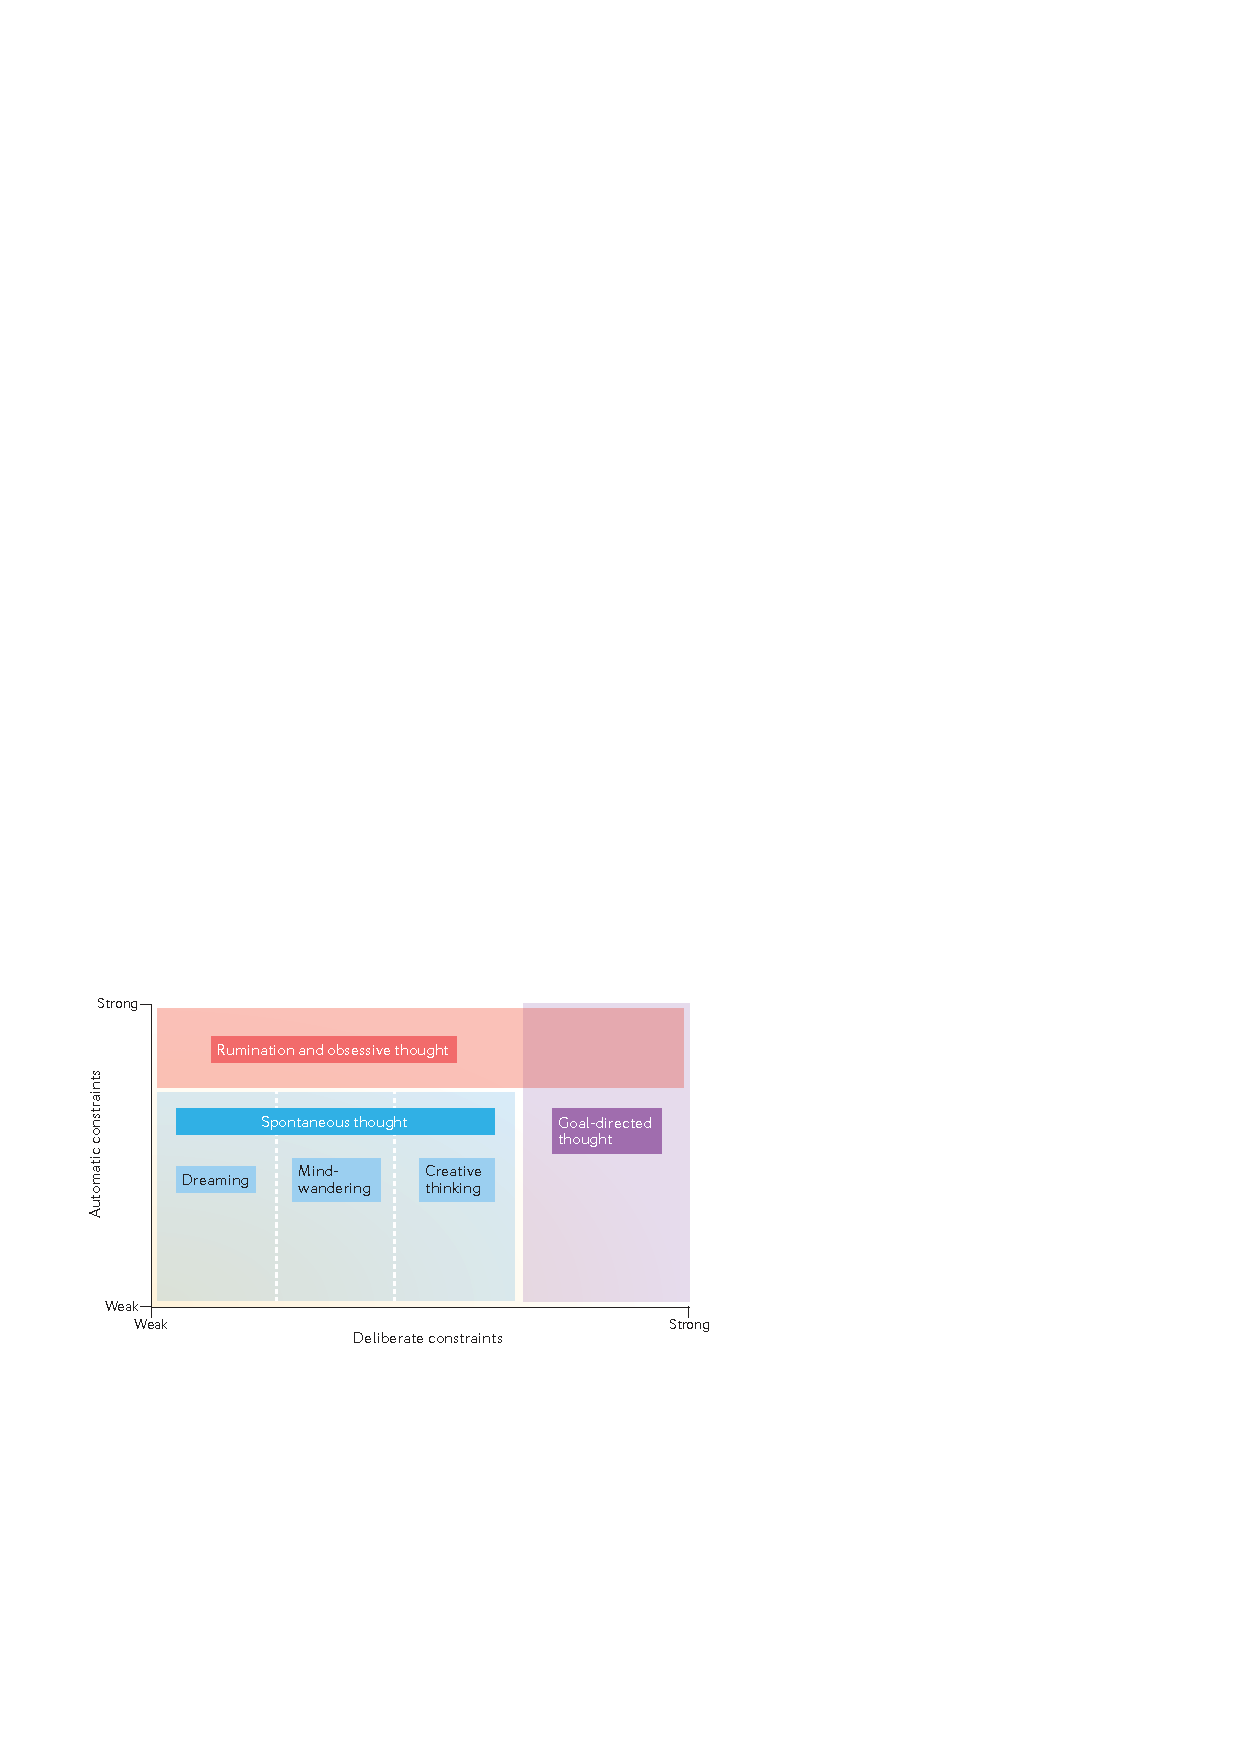
\includegraphics{assets/conceptual_space} 

}

\caption{Conceptual space of different types of thought (Christoff et al., 2016)}\label{fig:unnamed-chunk-1}
\end{figure}

\ldots{}

\chapter{Electromyographic correlates of speech
production}\label{electromyographic-correlates-of-speech-production}

\ldots{}

\section{Speech production
mechanisms}\label{speech-production-mechanisms}

\ldots{}

\section{Speech production muscles}\label{speech-production-muscles}

\ldots{}

\section{Muscular physiology}\label{muscular-physiology}

\ldots{}

\section{EMG signal}\label{emg-signal}

\subsection{EMG signal measures}\label{emg-signal-measures}

Muscular activity can be studied at different levels. At the cellular
level, using electrophysiological measures like micro-electrods
implanted in the cell, that allow direct measures of \textbf{action
potential}. At the segmental level, biomechanis study muscular activity
using surface sensors, positionned on the skin\ldots{}intermediate
levels\ldots{}

\subsection{Motor Unit Action
Potential}\label{motor-unit-action-potential}

\textbf{Motor unit action potential} (MUAP) is the electric field
resulting from the sum f the electric fiels emitted y each fiber of the
motor unit. This train of action potentials will generate a \emph{train}
of MUAP, call \textbf{motor unit action potential trains} (MUAPT). The
electric potential generated by this field is highly dependant of
parameters such as the number of fibers, their length, speed of
conduction and position of the neuromuscular junction.

\begin{figure}

{\centering 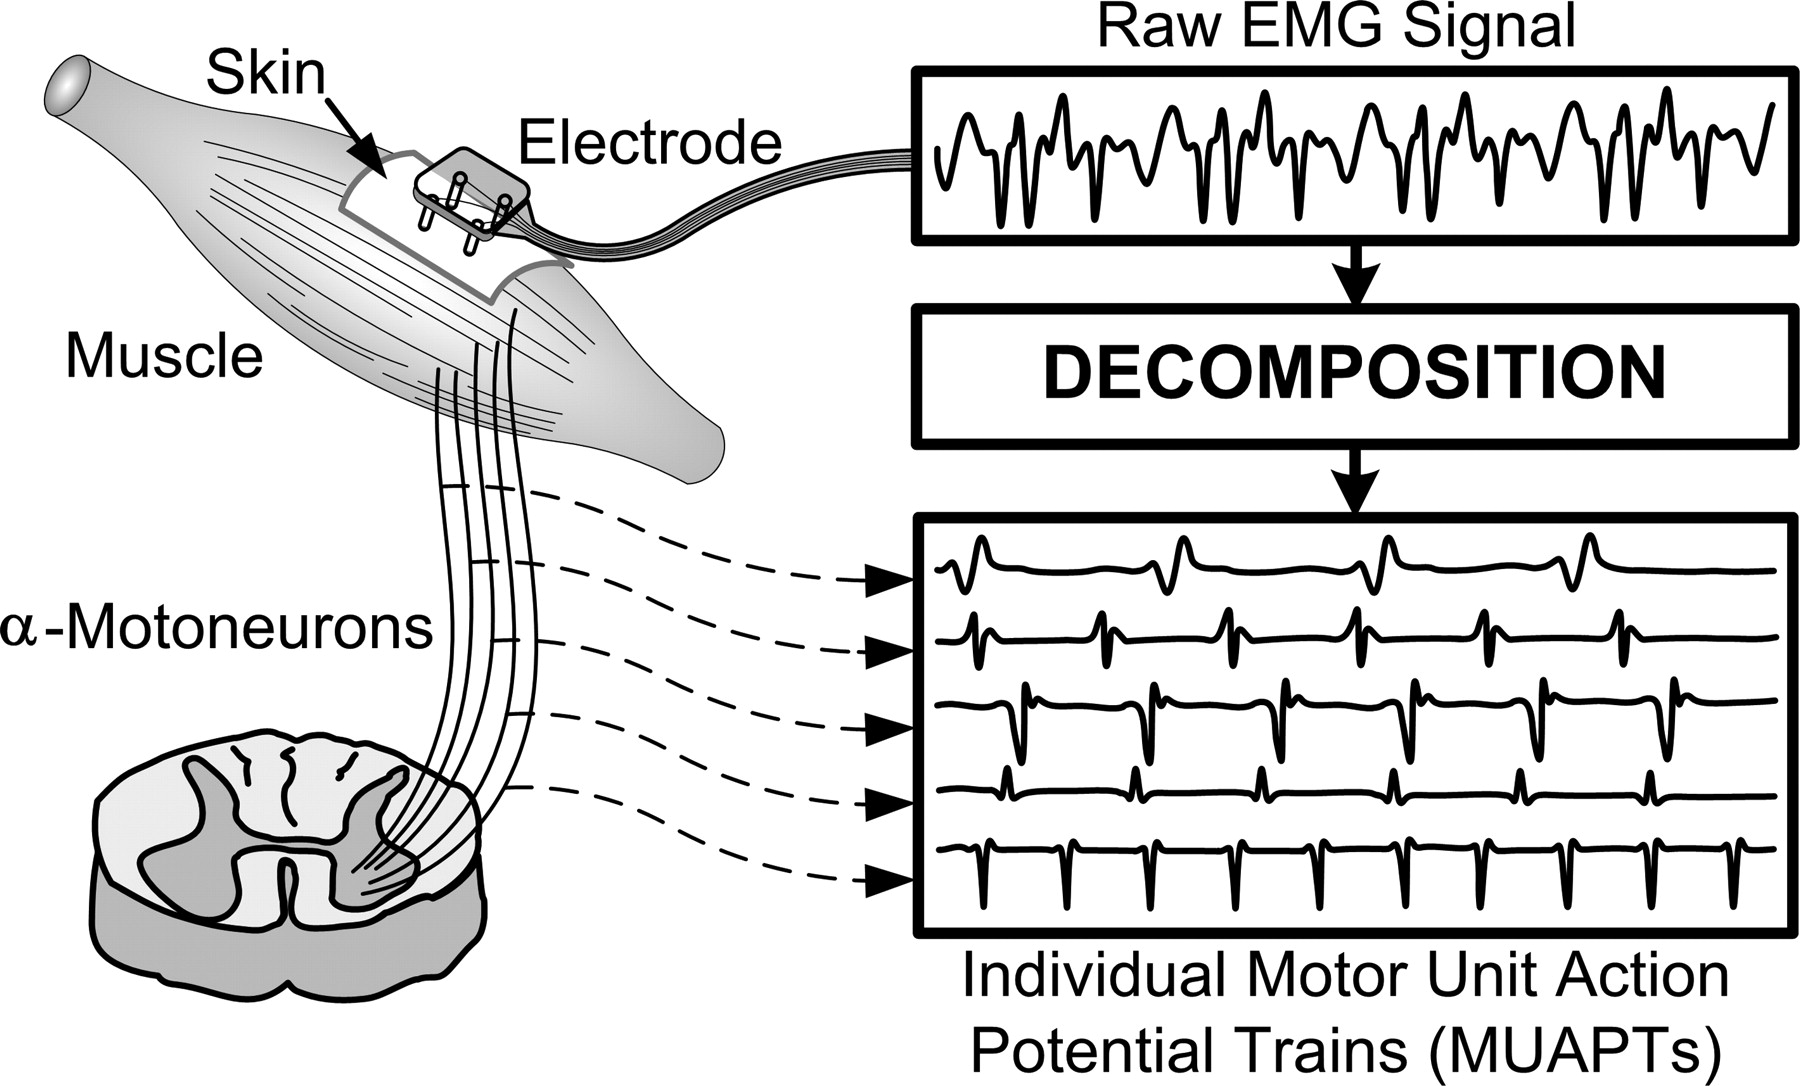
\includegraphics{assets/muap} 

}

\caption{Motor unit action potential schema.}\label{fig:unnamed-chunk-1}
\end{figure}

\ldots{}

EMG signal then result in a mixture of recruited motor units.

\subsection{Surface EMG}\label{surface-emg}

\ldots{}\emph{crosstalk} phenomenon \citep{DeLuca1997}. In reason of the
important\ldots{} of facial muscles, the EMG activity of one recorded
muscle generally does not represent the activity of a single muscle but
rather a mixture of\ldots{}\citet{Rapin2011}\ldots{}

\subsection{Basic signal processing}\label{basic-signal-processing}

\ldots{}the EMG signal is a stochastic signal\ldots{} In order to
illustrate what EMG signal looks like, we simulated EMG signal based on
a standard algorithm \citep[pp.70-71]{Hermens1999}, implemented in R by
\citet{Borg2014}.

\begin{Shaded}
\begin{Highlighting}[]
\OperatorTok{>}\StringTok{ }\KeywordTok{source}\NormalTok{(}\StringTok{"code/EMGfuns.R"}\NormalTok{)}
\OperatorTok{>}\StringTok{ }\NormalTok{emg <-}\StringTok{ }\KeywordTok{EMG_sim}\NormalTok{(}\DataTypeTok{n =} \DecValTok{2048}\NormalTok{, }\DataTypeTok{sampFreq =} \DecValTok{1000}\NormalTok{, }\DataTypeTok{lF =} \DecValTok{10}\NormalTok{, }\DataTypeTok{hF =} \DecValTok{100}\NormalTok{)}\OperatorTok{$}\NormalTok{sim}
\OperatorTok{>}\StringTok{ }\KeywordTok{ts.plot}\NormalTok{(emg, }\DataTypeTok{xlab =} \StringTok{"Time (ms)"}\NormalTok{, }\DataTypeTok{ylab =} \StringTok{"simEMG"}\NormalTok{, }\DataTypeTok{col =} \StringTok{"steelblue"}\NormalTok{)}
\end{Highlighting}
\end{Shaded}

\begin{figure}[h!]

{\centering 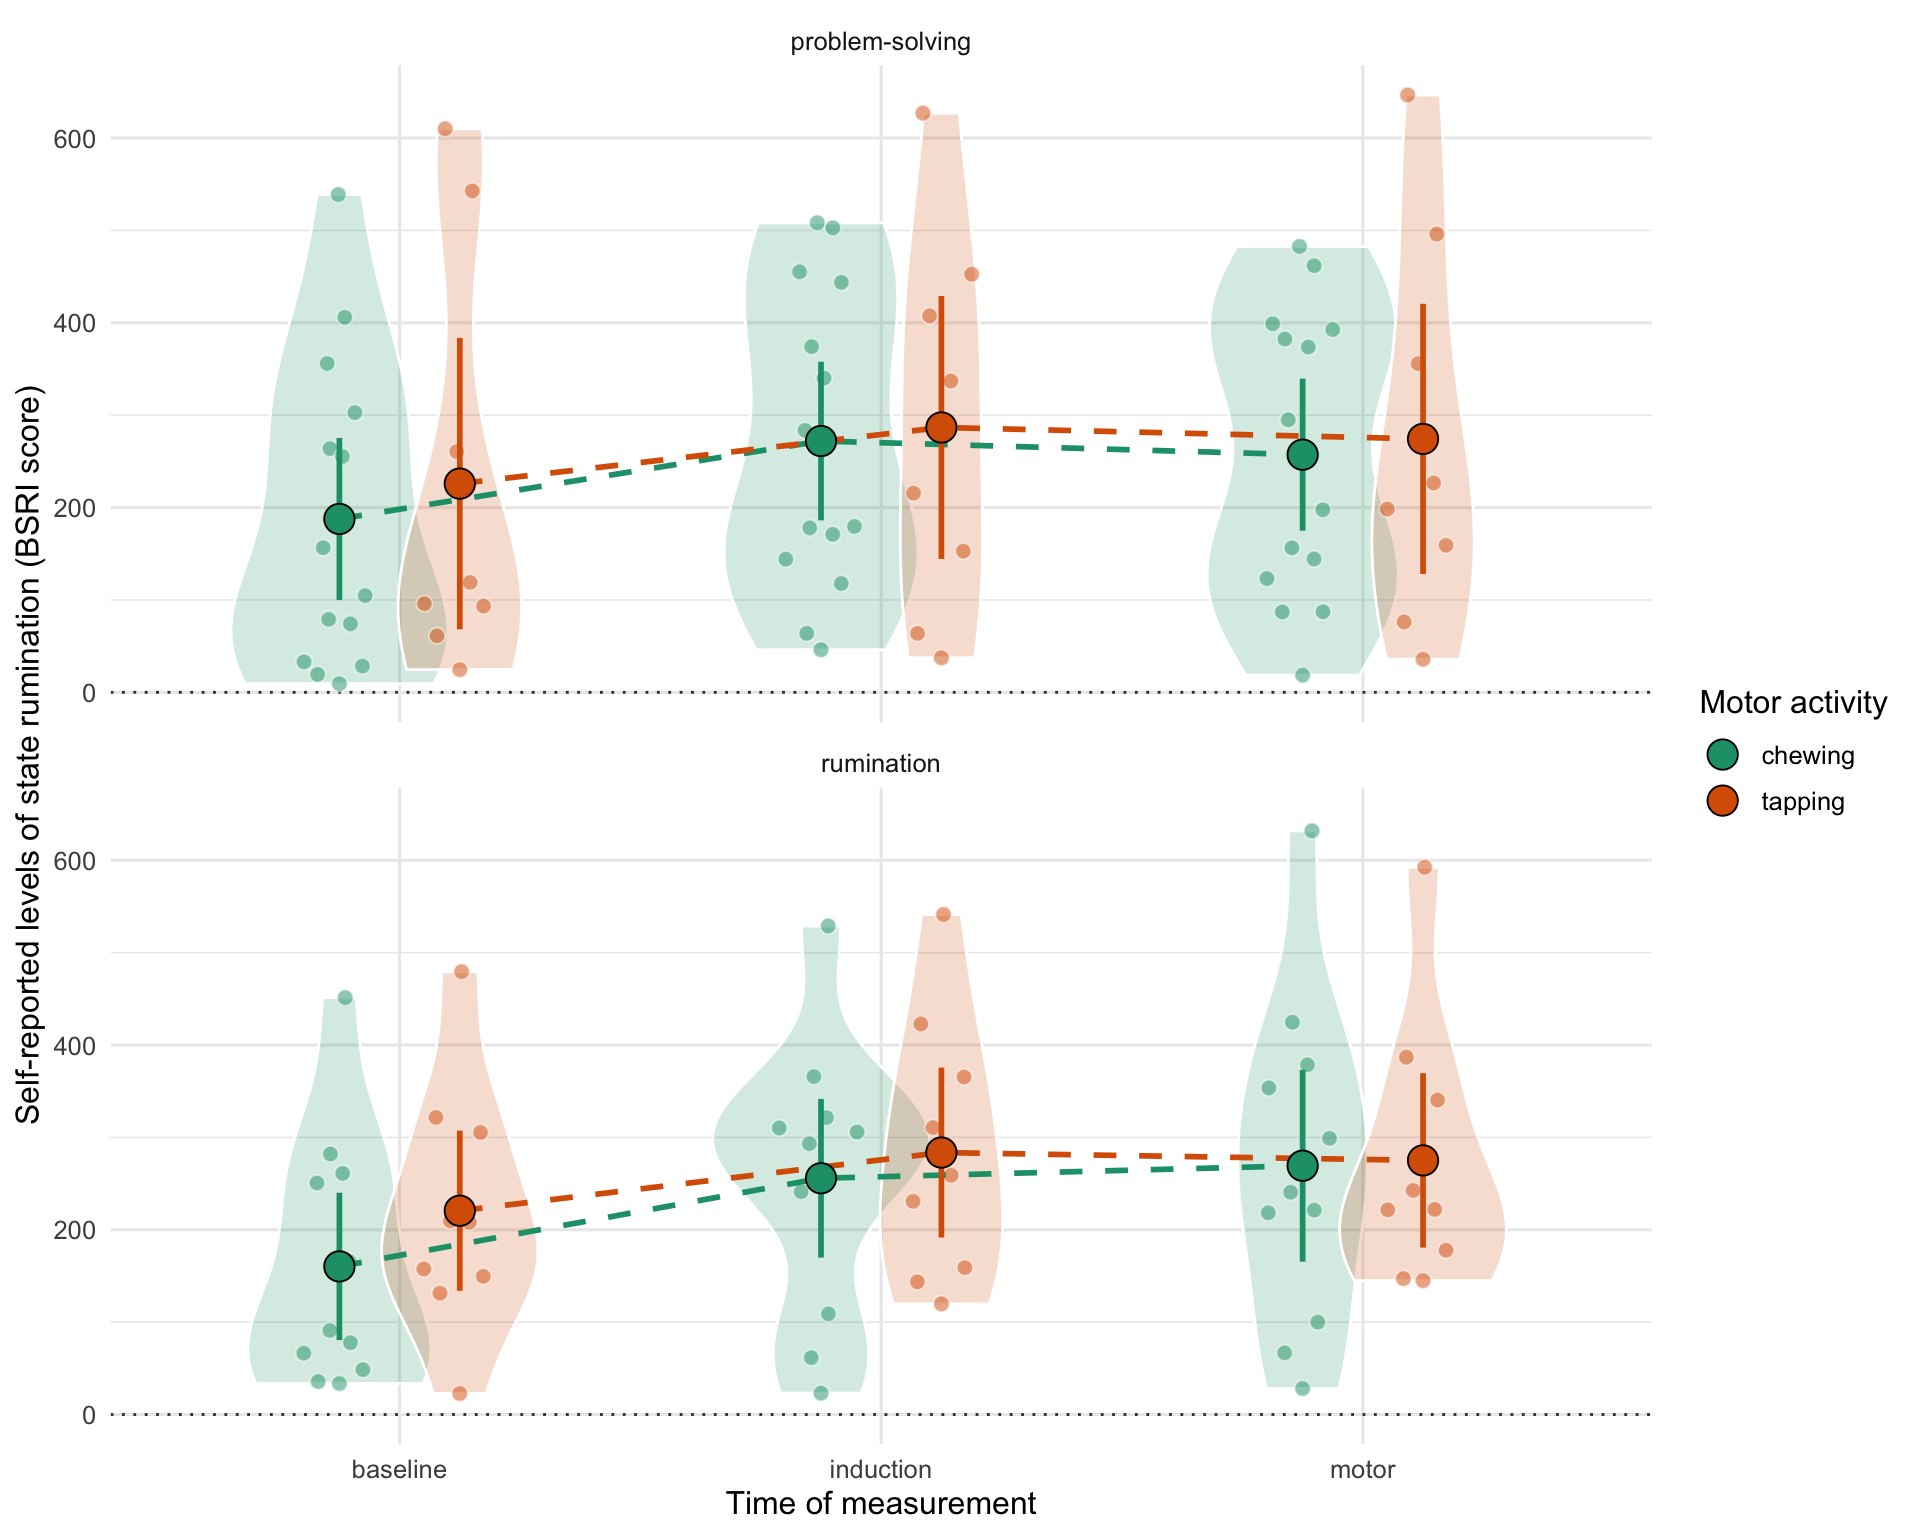
\includegraphics{02-chap2_files/figure-latex/unnamed-chunk-2-1} 

}

\caption{Simulated EMG signal.}\label{fig:unnamed-chunk-2}
\end{figure}

\ldots{}we rectify the EMG signal by taking its absolute value and
substracting the mean in order to correct for any offset (bias) present
in the raw data. It is interesting to note that the effects of
rectification on the EMG signal is similar to the rectification of AM
radio waves whose purpose is to enhance the low frequency components,
wich encode the voice signals. Concerning EMG, the ``voice'' of the
signal corresponds to the encoded force \citep{Borg2007}.

\begin{Shaded}
\begin{Highlighting}[]
\OperatorTok{>}\StringTok{ }\NormalTok{emg <-}\StringTok{ }\KeywordTok{abs}\NormalTok{(emg }\OperatorTok{-}\StringTok{ }\KeywordTok{mean}\NormalTok{(emg) )}
\OperatorTok{>}\StringTok{ }\KeywordTok{ts.plot}\NormalTok{(emg, }\DataTypeTok{xlab =} \StringTok{"Time (ms)"}\NormalTok{, }\DataTypeTok{ylab =} \StringTok{"simEMG"}\NormalTok{, }\DataTypeTok{col =} \StringTok{"steelblue"}\NormalTok{)}
\end{Highlighting}
\end{Shaded}

\begin{figure}[h!]

{\centering 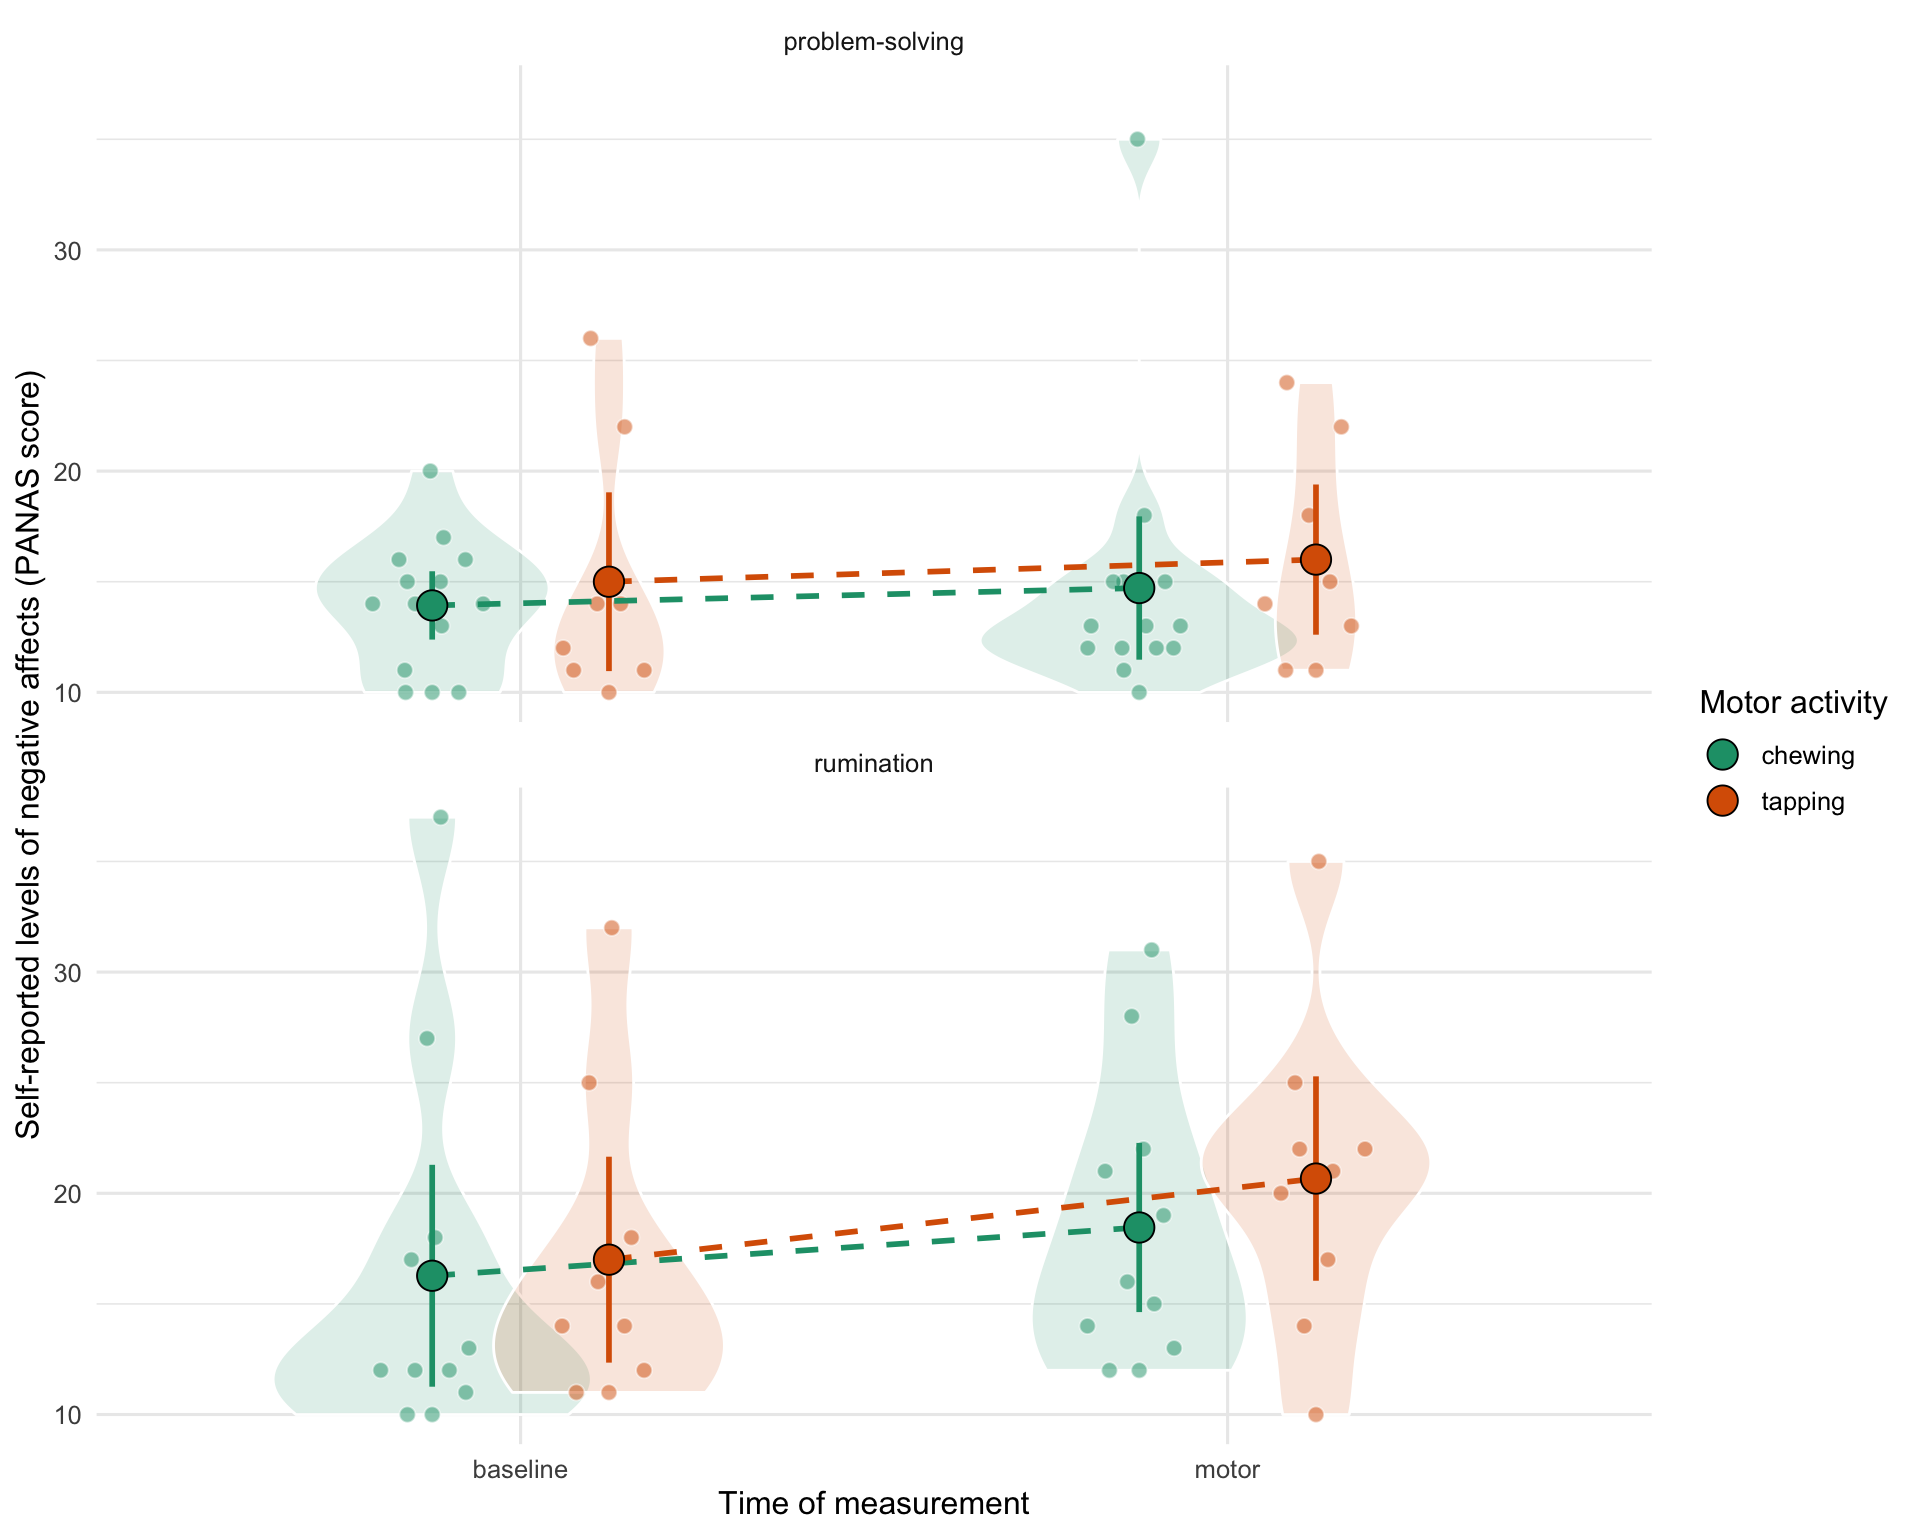
\includegraphics{02-chap2_files/figure-latex/unnamed-chunk-3-1} 

}

\caption{Rectified EMG signal.}\label{fig:unnamed-chunk-3}
\end{figure}

\ldots{}

There are two main measures thant can be used to represent the magnitude
of muscle activity. These two measures can be directly computed from the
filtered EMG signal. The first one is the \textbf{average rectified
value} (ARV):

\[ARV = \frac{1}{T} \sum_{t=1}^{T} | EMG(t_{i}) |\]

which is computed over a specific interval \((0,T)\) and where
\(|EMG(_{i})|\) is the absolute value of a datum of EMG in the data
window. The unit of measurement is \(mV\) or \(\mu V\), and the ARV
calculation is generally similar to the numerical formula for
integration \citep{Kamen2010}.

The second one is the \textbf{root-mean-square} (RMS) amplitude:

\[RMS = \sqrt \frac{1}{T} \sum_{t=1}^{T} | EMG^{2}(t_{i}) |\]

where \(|EMG^{2}(_{i})|\) is the squared value of each EMG datum and has
both physical and physiological meanings\ldots{}

\part{Experimental part}\label{part-experimental-part}

Blah blah blah\ldots{} explain why two parts\ldots{}

\chapter{Orofacial electromyographic correlates of induced verbal
rumination}\label{orofacial-electromyographic-correlates-of-induced-verbal-rumination}

Biological Psychology paper\ldots{}

\chapter{Dissociating facial electromyographic correlates of visual and
verbal induced
rumination}\label{dissociating-facial-electromyographic-correlates-of-visual-and-verbal-induced-rumination}

Second EMG study with Sonja\ldots{}

\chapter{Zygoto experiment}\label{zygoto-experiment}

\ldots{}

\chapter{Articulatory suppression effects on induced
rumination}\label{articulatory-suppression-effects-on-induced-rumination}

Summary of the research\ldots{}\footnote{This experimental chapter is
  manuscript reformatted for the need of this thesis. Source: The
  manuscript has been submitted to Psychological Research.
  Pre-registered protocol, preprint, data, as well as reproducible code
  and figures are available at: \url{https://osf.io/3bh67/}.}

\section{Introduction}\label{introduction}

A large part of our inner experience involves verbal content, with
internal monologues and conversations. Inner speech is considered as a
major component of conscious experience and cognition
\citep{Hubbard2010, Klinger1987, Hurlburt2013}. An important issue
related to inner speech concerns its format and nature and whether it is
better described as a mere evocation of abstract amodal verbal
representations or as a concrete motor simulation of actual speech
production. In the first case, inner speech is seen as divorced from
bodily experience, and includes, at most, faded auditory
representations. In the second case, inner speech is considered as a
physical process that unfolds over time, leading to an enactive
re-creation of auditory a well as articulatory percepts. The latter
hypothesis is interesting in the context of persistent negative and
maladaptive forms of inner speech, such as rumination. If this
hypothesis is correct, we could expect rumination --as a particular type
of inner speech-- to be disrupted by concurrent involvement of the
speech muscles.

\subsection{Multisensory and motor components of inner
speech}\label{multisensory-and-motor-components-of-inner-speech}

Introspective explorations of the characteristics of inner speech have
led to different views on the relative importance of its auditory and
articulatory components, and on the involvement of motor processes. For
\citet{Stricker1880}, ``speech representations are motor
representations'', while \citet{Egger1881} believed that auditory
representations are dominant in inner speech and that motor
representations are not always present. However, as noted by
\citet{Ballet1886}, these contradictory hypotheses might stem from an
over-generalization of their own introspective findings, the former
discovering motor feelings and the latter auditory images
\citep{Ballet1886}. In the same vein, \citet{Paulhan1886} claimed that
inner speech involves both auditory and motor images, defining motor
images as the sensations in the speech organs (larynx, tongue, lips)
that sometimes accompany inner speech. Therefore, Paulhan's notion of
\emph{motor images} are in fact related to somatosensory representations
rather than to the involvement of actual speech movements (as claimed by
Stricker). It remains, however, that a distinction was introduced by
19th century authors between sensory and motor phenomena in inner
speech, with sensory phenomena including auditory as well as
articulatory (or somatosensory) percepts. The intuitive distinction
between auditory and motor phenomena is referred to in contemporary
research by the terms of \emph{inner ear} and \emph{inner voice}, in
line with Baddeley's classic model of working memory
\citetext{\citealp[e.g.,][]{Baddeley1974}; \citealp[see
also][]{Buchsbaum2013}}. Baddeley's model relies on a partnership
between an \emph{inner ear} (i.e., storage) and an \emph{inner voice}
\citep[i.e., subvocal rehearsal; see][]{Smith1995}.

Empirical arguments supporting the crucial role of the inner voice in
verbal memory (subvocal rehearsal) and auditory imagery can be found in
studies using articulatory suppression, in which the \emph{action}
component (i.e., the \emph{inner voice}) of inner speech is disrupted.
Articulatory suppression usually refers to a task which requires
participants to utter speech sounds (or to produce speech gestures
without sound), so that this activity disrupts ongoing speech production
processes. Articulatory suppression can be produced with different
degrees of vocalisation, going from overt uttering of irrelevant words,
to whispering, mouthing (i.e., silent articulation), and simple clamping
of the speech articulators. Many verbal working memory studies have
shown that articulatory suppression impairs recall performance
\citep[e.g.,][]{Baddeley1984}.

In a study aiming at investigating the role of \emph{covert enactment}
in auditory imagery, \citet{Reisberg1989} observed that the verbal
transformation effect \citep[VTE,][]{Warren1958}, namely the alteration
of speech percepts when certain speech sounds are uttered in a
repetitive way, also occurred during inner speech (although the VTE was
smaller than during overt speech), but was suppressed by concurrent
articulation (e.g., chewing) or clamping the articulators. The fact that
the VTE was observed during inner speech and that it was reduced by
concurrent chewing, even in inner speech, speaks in favour of the view
of inner speech as an enacted simulation of overt speech.

Another piece of evidence for the effect of articulatory suppression on
inner speech comes from a recent study by \citet{Topolinski2009} on the
mere exposure effect, namely the fact that repeated exposure to a
stimulus influences the evaluation of this stimulus in a positive way
\citep{Zajonc1968}. Topolinski and Strack's study showed that the mere
exposure effect for visually presented verbal material could be
completely suppressed by blocking subvocal rehearsal (i.e., inner
speech) when asking participants to chew a gum. The effect was
preserved, however, when participants kneaded a soft ball with their
hand \citep{Topolinski2009}. This finding suggests that blocking speech
motor simulation interfered with the inner rehearsal of the visually
presented verbal stimuli, thereby destroying the positive exposure
effect. It provides additional experimental support to the view that
inner speech involves a motor component.

The occurrence of motor simulation during inner speech is further backed
by several studies using physiological measures to evaluate inner speech
production properties. Using electrodes inserted in the tongue tip or
lips of five participants, \citet{Jacobson1931} was able to detect
electromyographic (EMG) activity during several tasks requiring inner
speech. Similarly, \citet{Sokolov1972} recorded intense lip and tongue
muscle activation when participants had to perform complex tasks that
necessitated substantial inner speech production (e.g., problem
solving). Another study using surface electromyography (sEMG)
demonstrated an increase in activity of the lip muscles during silent
recitation tasks compared to rest, but no increase during the
non-linguistic visualisation task \citep{Livesay1996}. An increase in
the lip and forehead muscular activity has also been observed during
induced rumination \citep{Nalborczyk2017}. Furthermore, this last study
also suggested that speech-related muscle relaxation was slightly more
efficient in reducing subjective levels of rumination than non
speech-related muscle relaxation, suggesting that relaxing or inhibiting
the speech muscles could disrupt rumination.

\subsection{Rumination}\label{rumination}

Rumination is a ``class of conscious thoughts that revolve around a
common instrumental theme and that recur in the absence of immediate
environmental demands requiring the thoughts'' \citep{Martin1996}.
Despite the fact that depressed patients report positive metacognitive
beliefs about ruminating, which is often seen as a coping strategy in
order to regulate mood \citep[e.g.,][]{Papageorgiou2001}, rumination is
known to significantly worsen mood
\citep[e.g.,][]{Moberly2008, Nolen-hoeksema1993}, impair cognitive
flexibility \citep[e.g.,][]{Davis2000, Lyubomirsky1998}, and to lead
toward pronounced social exclusion and more interpersonnal distress
\citep{Lam2003}. Although partly visual, rumination is a predominantly
verbal process \citep{Goldwin2012, Mclaughlin2007} and can be considered
as a maladaptive type of inner speech.

In a study on worry, another form of repetitive negative thinking,
\citet{Rapee1993} observed a \emph{tendency} for articulatory
suppression, but not for visuo-spatial tasks, to produce some
interference with worrying. He concluded that worry involves the
phonological aspect of the central executive of working memory. We
further add that, since repeating a word seems to reduce the ability to
worry, this study suggests that articulatory aspects are at play during
worry.

In this context, the question we addressed in this study is whether
verbal rumination consists of purely abstract verbal representations or
whether it is better described as a motor simulation of speech
production, engaging the speech apparatus. If the latter hypothesis is
correct, rumination experienced in verbal form (in contrast to a
non-verbal form) should be disrupted by mouthing (i.e., silent
articulation), and should not be disrupted by a control task that does
not involve speech muscles (e.g., finger-tapping). Specifically, we thus
sought to test the hypotheses that rumination could be disrupted by
articulatory suppression (but not by finger-tapping), and that this
disruption would be more pronounced when rumination is experienced in a
verbal form than in a non-verbal form.

\section{Methods}\label{methods}

In the \emph{Methods} and \emph{Data analysis} sections, we report how
we determined our sample size, all data exclusions, all manipulations,
and all measures in the study \citep{Simmons2012}. A pre-registered
version of our protocol can be found on OSF:
\url{https://osf.io/3bh67/}.

\subsection{Sample}\label{sample}

We originally planned for 128 participants to take part in the study.
This sample size was set on the basis of results obtained by
\citet{Topolinski2009}, who observed an effect size around
\(\eta_{p}^{2}=.06\). We expected a similar effect size for the current
rumination disruption, since rumination can be conceived of as a subtype
of inner speech\footnote{In the original power calculations included in
  the OSF preregistration platform, we had inadequately specified the
  effect size in GPower, but we only realised this erroneous
  specification after the freezing of the preregistration on the OSF
  platform. Therefore, the current sample size slightly differs from the
  preregistered one.}.

As we anticipated drop-out of participants due to our inclusion criteria
(see below), a total of 184 undergraduate students in psychology from
the Université Grenoble Alpes took part in this experiment, in exchange
for course credits. They were recruited via mailing list, online student
groups, and posters. Each participant provided a written consent and
this study was approved by the local ethics committee (CERNI N°
2016-05-31-9). To be eligible, participants had to be between 18 and 35
years of age, with no history of motor, neurological, psychiatric, or
speech-development disorders. All participants spoke French as their
mother tongue. After each participant gave their written consent, they
completed the Center for Epidemiologic Studies - Depression scale
\citep[CES-D;][]{Radloff1977a}. The CES-D is a 12-item questionnaire,
validated in French \citep{Morin2011}, aiming to assess the level of
depressive symptoms in a subclinical population. Participants exceeding
the threshold of clinical depressive symptoms \citep[i.e.,
\textgreater{}23 for females and \textgreater{}17 for
males;][]{Radloff1977a} were not included in the study for ethical
reasons (N = 26).

To investigate articulatory suppression effects in the context of
rumination, a successful induction of rumination is a prerequisite.
Therefore, analyses were only conducted on participants who showed an
effect of the rumination induction (i.e., strictly speaking,
participants who reported more rumination after the induction than
before). We thus discarded participants who did not show any increase in
rumination level (N = 52, 32.91\% of total sample). The final sample
comprised 106 participants (Mean age = 20.3018868, SD = 2.5728064,
Min-Max = 18-31, 96 females).

\subsection{Material}\label{material}

The experiment was programmed with OpenSesame software
\citep{Mathot2012} and stimuli were displayed on a DELL latitude E6500
computer screen.

\subsubsection{Questionaires}\label{questionaires}

To control for confounding variables likely to be related to the
intensity of the induction procedure, we administered the French version
of the Positive and Negative Affect Schedule
\citep[PANAS;][]{Watson1988}, adapted to French by \citet{Gaudreau2006}.
This questionnaire includes 20 items, from which we can compute an
overall index of both positive (by summing the scores on 10 positive
items, thereafter \emph{PANASpos}) and negative affect (\emph{PANASneg})
at baseline. This questionnaire was administered at baseline. In order
to evaluate trait rumination, at the end of the experiment participants
completed the short version of the Ruminative Response Scale
\citep[RRS-R,][]{Treynor2003}, validated in French (Douilliez, Guimpel,
Baeyens, \& Philippot, \emph{in preparation}). From this questionnaire,
scores on two dimensions were analysed (\emph{RRSbrooding} and
\emph{RRSreflection}).

\subsubsection{Measures}\label{measures}

Measures of state rumination were recorded using a Visual Analogue Scale
(VAS) previously used in \citet{Nalborczyk2017}. This scale measured the
degree of agreement with the sentence ``At this moment, I am brooding on
negative things'' (translated from French), on a continuum between ``Not
at all'' and ``A lot'' (afterwards coded between 0 and 100). This scale
is subsequently referred to as the \emph{RUM} scale. It was used three
times in the experiment, at baseline (after training but before the
experiment started), after rumination induction, and after a motor task.

Additionally, participants answered questions about the modality of the
thoughts that occurred while performing the motor task. This last
questionnaire consisted of one question evaluating the occurrence
frequency of different modalities of inner thoughts (e.g., visual
imagery, verbal thoughts, music). Then, a verbal/non-verbal ratio (i.e.,
the score on the verbal item divided by the mean of the score on the
non-verbal items) was computed, hereafter referred to as the
\emph{Verbality} continuous predictor (this scale is available online:
\url{https://osf.io/3bh67/}).

\subsubsection{Tasks}\label{tasks}

In the first part of the experiment, ruminative thoughts were induced
using a classical induction procedure. Then a motor task was executed.
Participants were randomly allocated to one of two conditions. In the
\emph{Mouthing} condition, the task consisted of repetitively making
mouth opening-closing movements at a comfortable pace. This condition
was selected as it is commonly used in articulatory suppression studies
\citep[e.g.,][]{Baddeley1984}. As a control, a finger-tapping condition
was used (the \emph{Tapping} condition), that consisted of tapping on
the desk with the index finger of the dominant hand at a comfortable
pace.

Although finger-tapping tasks are generally considered as good control
conditions when using speech motor tasks, since they are comparable in
terms of general attentional demands, it may be that orofacial gestures
are intrinsically more complex than manual gestures \citep[i.e., more
costly,][]{Emerson2003}. To discard the possibility that orofacial
gestures (related to the \emph{Mouthing} condition) would be cognitively
more demanding than manual ones (related to the \emph{Tapping}
condition), we designed a pretest experiment in order to compare the two
interference motor tasks used in the main experiment. Results of this
control experiment showed no difference on reaction times during a
visual search task between the two interference tasks (i.e., mouthing
and finger-tapping). Full details are provided in Appendix A.

\subsection{Procedure}\label{procedure}

The experiment took place individually in a quiet and dimmed room. The
total duration of the session ranged between 35min and 40min. Before
starting the experiment, participants were asked to perform the motor
task during 1 min, while following a dot moving at a random pace on the
screen in front of them. This task was designed to train the
participants to perform the motor task adequately. Following this
training and after describing the experiment, the experimenter left the
room and each participant had to fill-in a baseline questionnaire
(adaptation of PANAS, see above) presented on the computer screen.
Baseline state rumination was then evaluated using the \emph{RUM} scale.
The whole experiment was video-monitored using a Sony HDR-CX240E video
camera, in order to check that the participants effectively completed
the task.

\subsubsection{Rumination induction}\label{rumination-induction}

Rumination induction consisted of two steps. The first step consisted of
inducing a negative mood in order to enhance the effects of the
subsequent rumination induction. Participants were asked to recall a
significant personal failure experienced in the past five years. Then,
participants were invited to evaluate the extent to which this memory
was ``intense for them'' on a VAS between ``Not at all'' and ``A lot'',
afterwards coded between 0 and 100, and referred to as \emph{Vividness}.

The second step consisted of the rumination induction proper. We used a
French translation of the \citet{Nolen-hoeksema1993} rumination
induction procedure. Participants had to read a list of 44 sentences
related to the meaning, the causes and the consequences of their current
affective or physiological state. Each phrase was presented on a
computer screen for 10 seconds and the total duration of this step was 7
minutes and 20 seconds. State rumination was then evaluated again using
the same VAS as the one used at baseline (\emph{RUM}).

\subsubsection{Motor task}\label{proc_supp}

After the rumination induction, participants were asked to continue to
think about ``the meaning, causes, and consequences'' of their feelings
while either repetitively making mouth movements (for participants
allocated in the ``Mouthing'' condition) or finger-tapping with the
dominant hand for five minutes (for participants allocated in the
``Tapping'' condition). Afterwards, state rumination was again evaluated
using the \emph{RUM} scale.

In order to evaluate trait rumination, participants completed the short
version of the RRS (see above). Then were filled in the questionnaire on
the modality of the thoughts that occurred while performing the motor
task (see above). Figure \ref{fig:diagram} summarises the full
procedure.

\begin{figure}[H]

{\centering 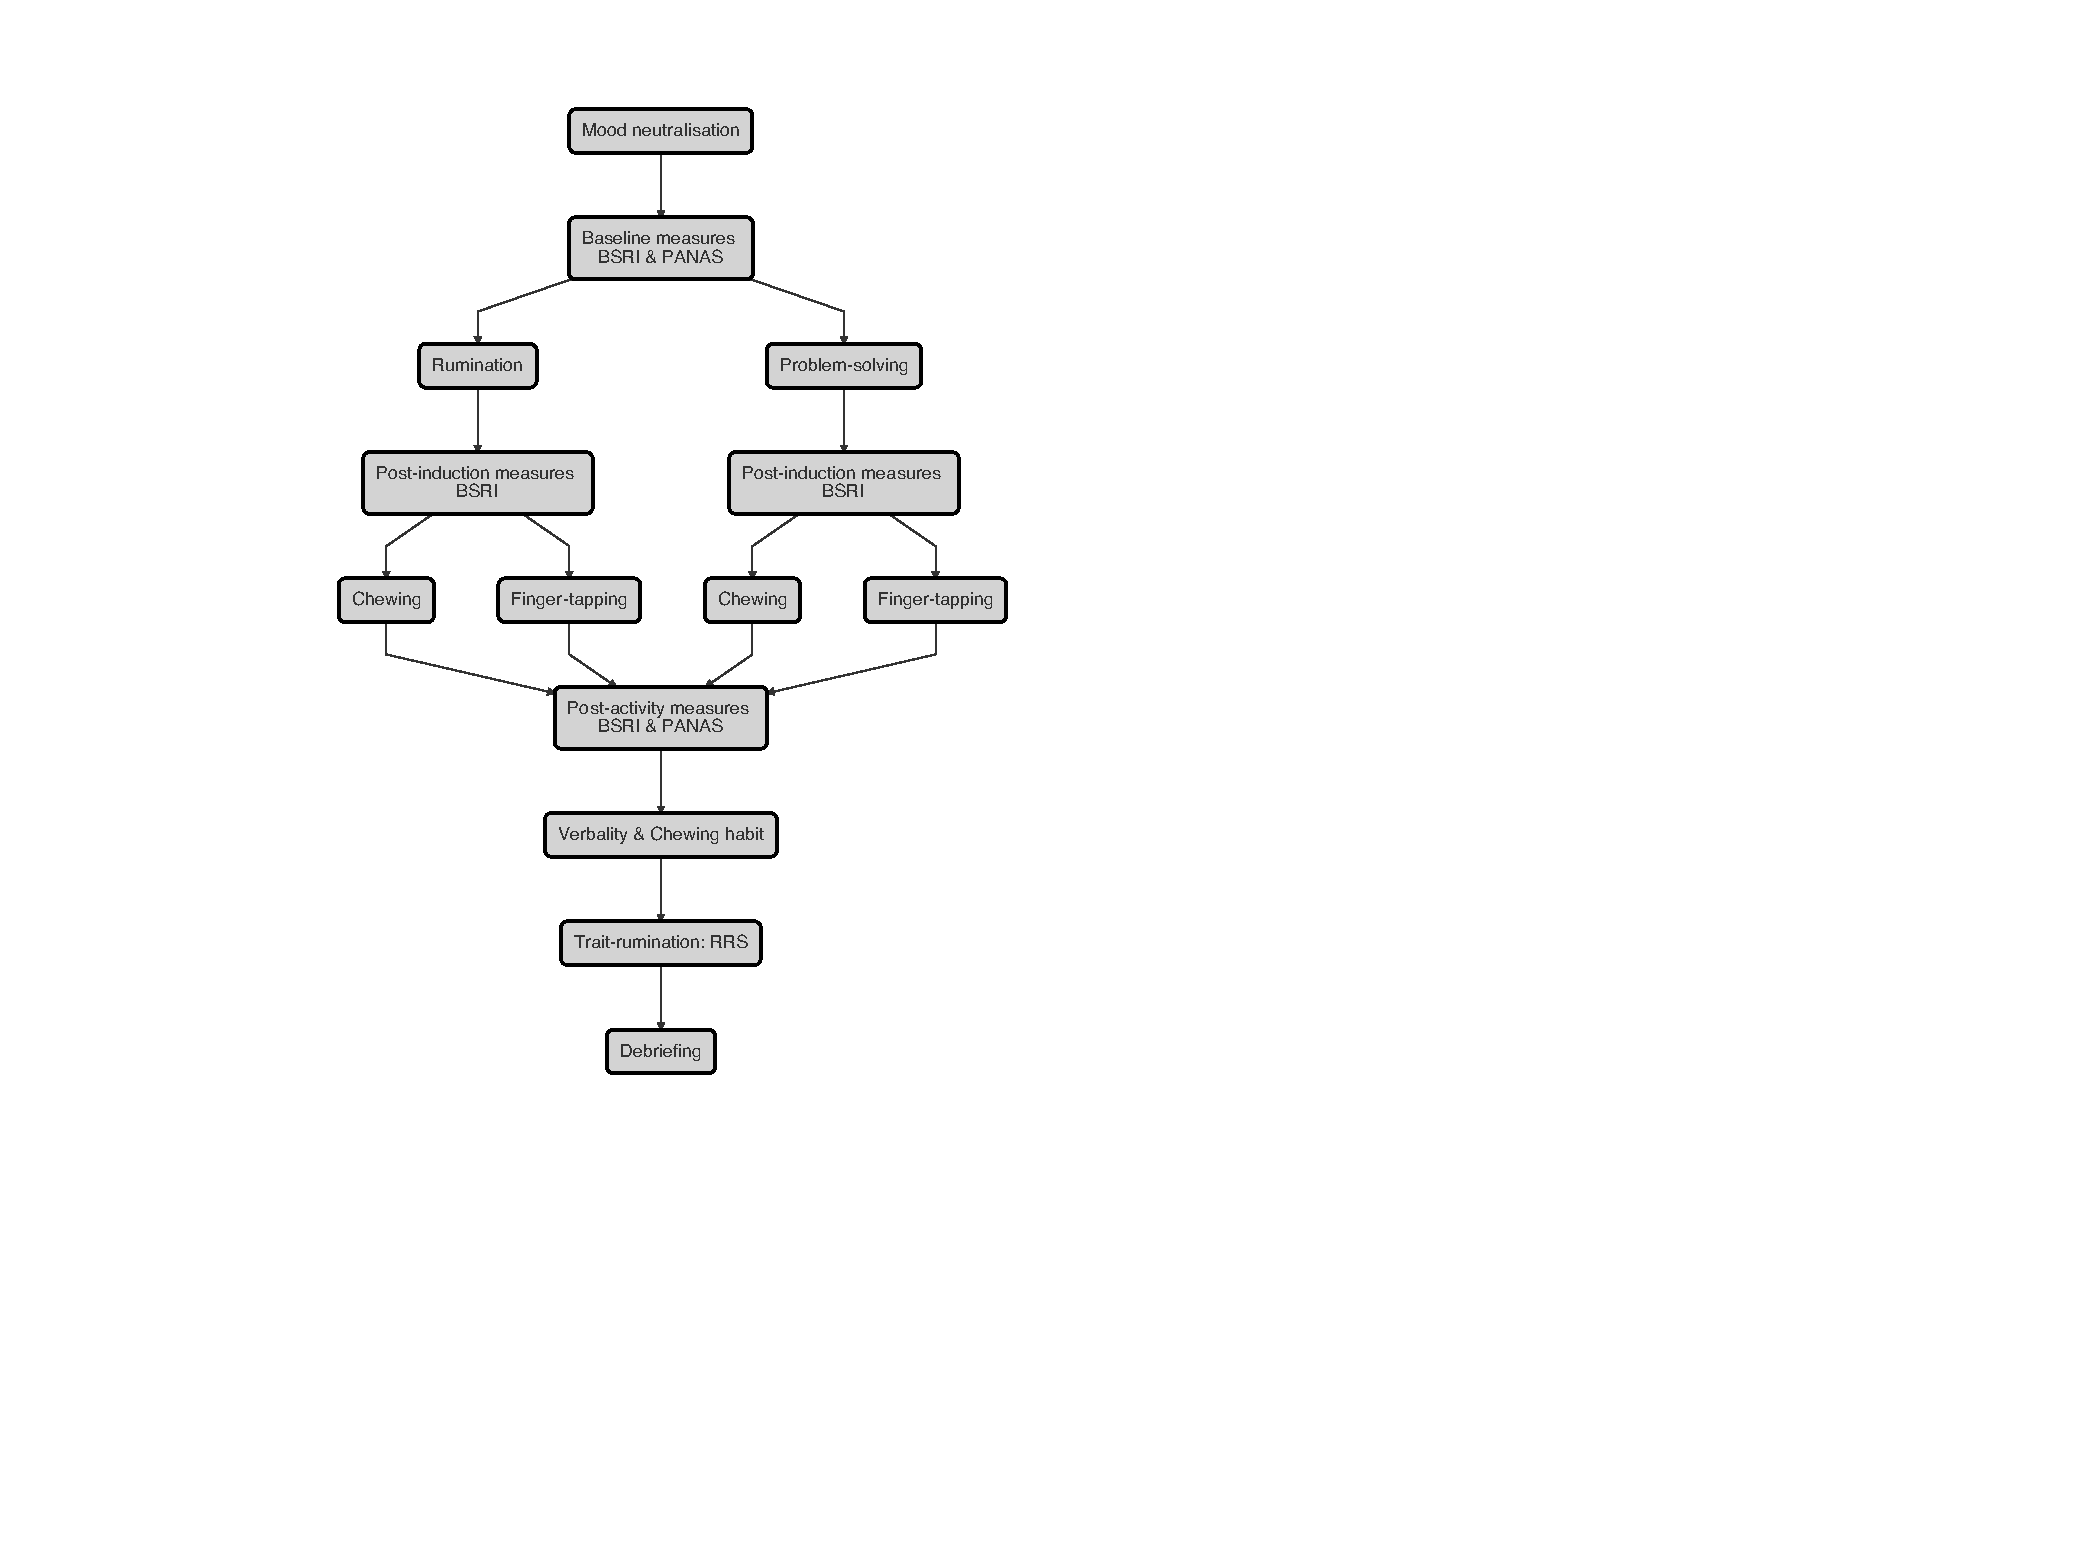
\includegraphics{06-chap6_files/figure-latex/diagram-1} 

}

\caption{Timeline of the experiment, from top to bottom.}\label{fig:diagram}
\end{figure}

\subsection{Data analysis}\label{data-analysis}

Statistical analyses were conducted using R version 3.4.3
\citep{R-base}, and are reported with the \texttt{papaja}
\citep{R-papaja} and \texttt{knitr} \citep{R-knitr} packages.

\subsubsection{Rumination induction}\label{rumination-induction-1}

We centered and standardised each predictor in order to facilitate the
interpretation of parameters. Data were then analysed using
\emph{Induction} (2 modalities, before and after induction,
contrast-coded) as a within-subject categorical predictor and \emph{RUM}
as a dependent variable in a multilevel linear model (MLM). Data were
fitted using the \texttt{lmer} function, within the \texttt{lme4}
package \citep{lme4}. This model was compared with more complex models
including effects of control variables, such as baseline affect state
(\emph{PANAS} scores) or the vividness of the memory chosen during the
induction (\emph{Vividness} score). Models were compared using the
corrected Akaike Information Criterion (AICc) and evidence ratios
\citep{Burnham2002, Burnham2011, Hegyi2011}. AICc provides a relative
measure of predictive accuracy of the models (the AIC is an
approximation of the out-of-sample deviance of a model) and balances
underfitting and overfitting by sanctioning models for their number of
parameters. We computed the difference between the best (lower) and
other AICcs with \(\Delta_{AICc}=AICc_{i}-AICc_{min}\) and then
expressed the weight of a model as:

\[w_{i}=\dfrac{exp(-\Delta_{i}/2)}{\sum_{r=1}^{R}exp(-\Delta_{r}/2)}\]

From there, we computed evidence ratios (ERs) as the ratios of weights:
\(ER_{ij} = \dfrac{w_{i}}{w_{j}}\), where \(w_{i}\) and \(w_{j}\) are
the Akaike weights of models \(i\) and \(j\), respectively. These
weights can be interpreted as the probability of the model being the
best model in terms of out-of-sample prediction \citep{Burnham2002}.
Instead of reporting null-hypothesis tests for our MLMs, we report 95\%
confidence intervals for the constant effects estimates\footnote{These
  may be interpreted as tests of significance: if the confidence
  interval for an estimated parameter does not contain zero, this
  estimate may be considered significant at \(\alpha\) \textless{}.05.}.

Whereas the use of AICc is appropriate for model comparison and
selection, it tells us nothing about the absolute fit of the model. To
estimate this fit, we computed two types of \(R^2\) for MLMs using the
\texttt{MuMIn} package \citep{MuMIn}. The first, called the marginal
\(R^2\) (\(R^2_{marg.}\)), estimates the proportion of variance
accounted for by the constant effects, whereas the second, called the
conditional \(R^2\) (\(R^2_{cond.}\)), estimates the proportion of
variance accounted for by the constant and the varying effects taken
together \citep{Getz2015, Johnson2014, Nakagawa2013}.

\subsubsection{Articulatory suppression
effects}\label{articulatory-suppression-effects}

Data were analysed in the same fashion as in the first part of the
experiment, using \emph{Session} (2 modalities, before and after motor
activity, contrast-coded) as a within-subject categorical predictor, and
\emph{Condition} (2 modalities, Mouthing and Tapping) as a
between-subject categorical predictor and \emph{RUM} as a dependent
variable, in a MLM.

\section{Results}\label{results}

\subsection{Correlation matrix between main predictors and control
variables}\label{correlation-matrix-between-main-predictors-and-control-variables}

In order to prevent multicollinearity, we estimated the correlation
between each pair of continuous predictors. Figure \ref{fig:correxp1}
displays these correlations along with the marginal distribution of each
variable. The absence of strong correlations (\(r > 0.8\)) between any
of these variables suggests that they can each be included as control
variables in the following statistical models. Summary statistics (mean
and standard deviation) for all these variables can be found in Table
\ref{tab:sumstat}.

\begin{figure}
\centering
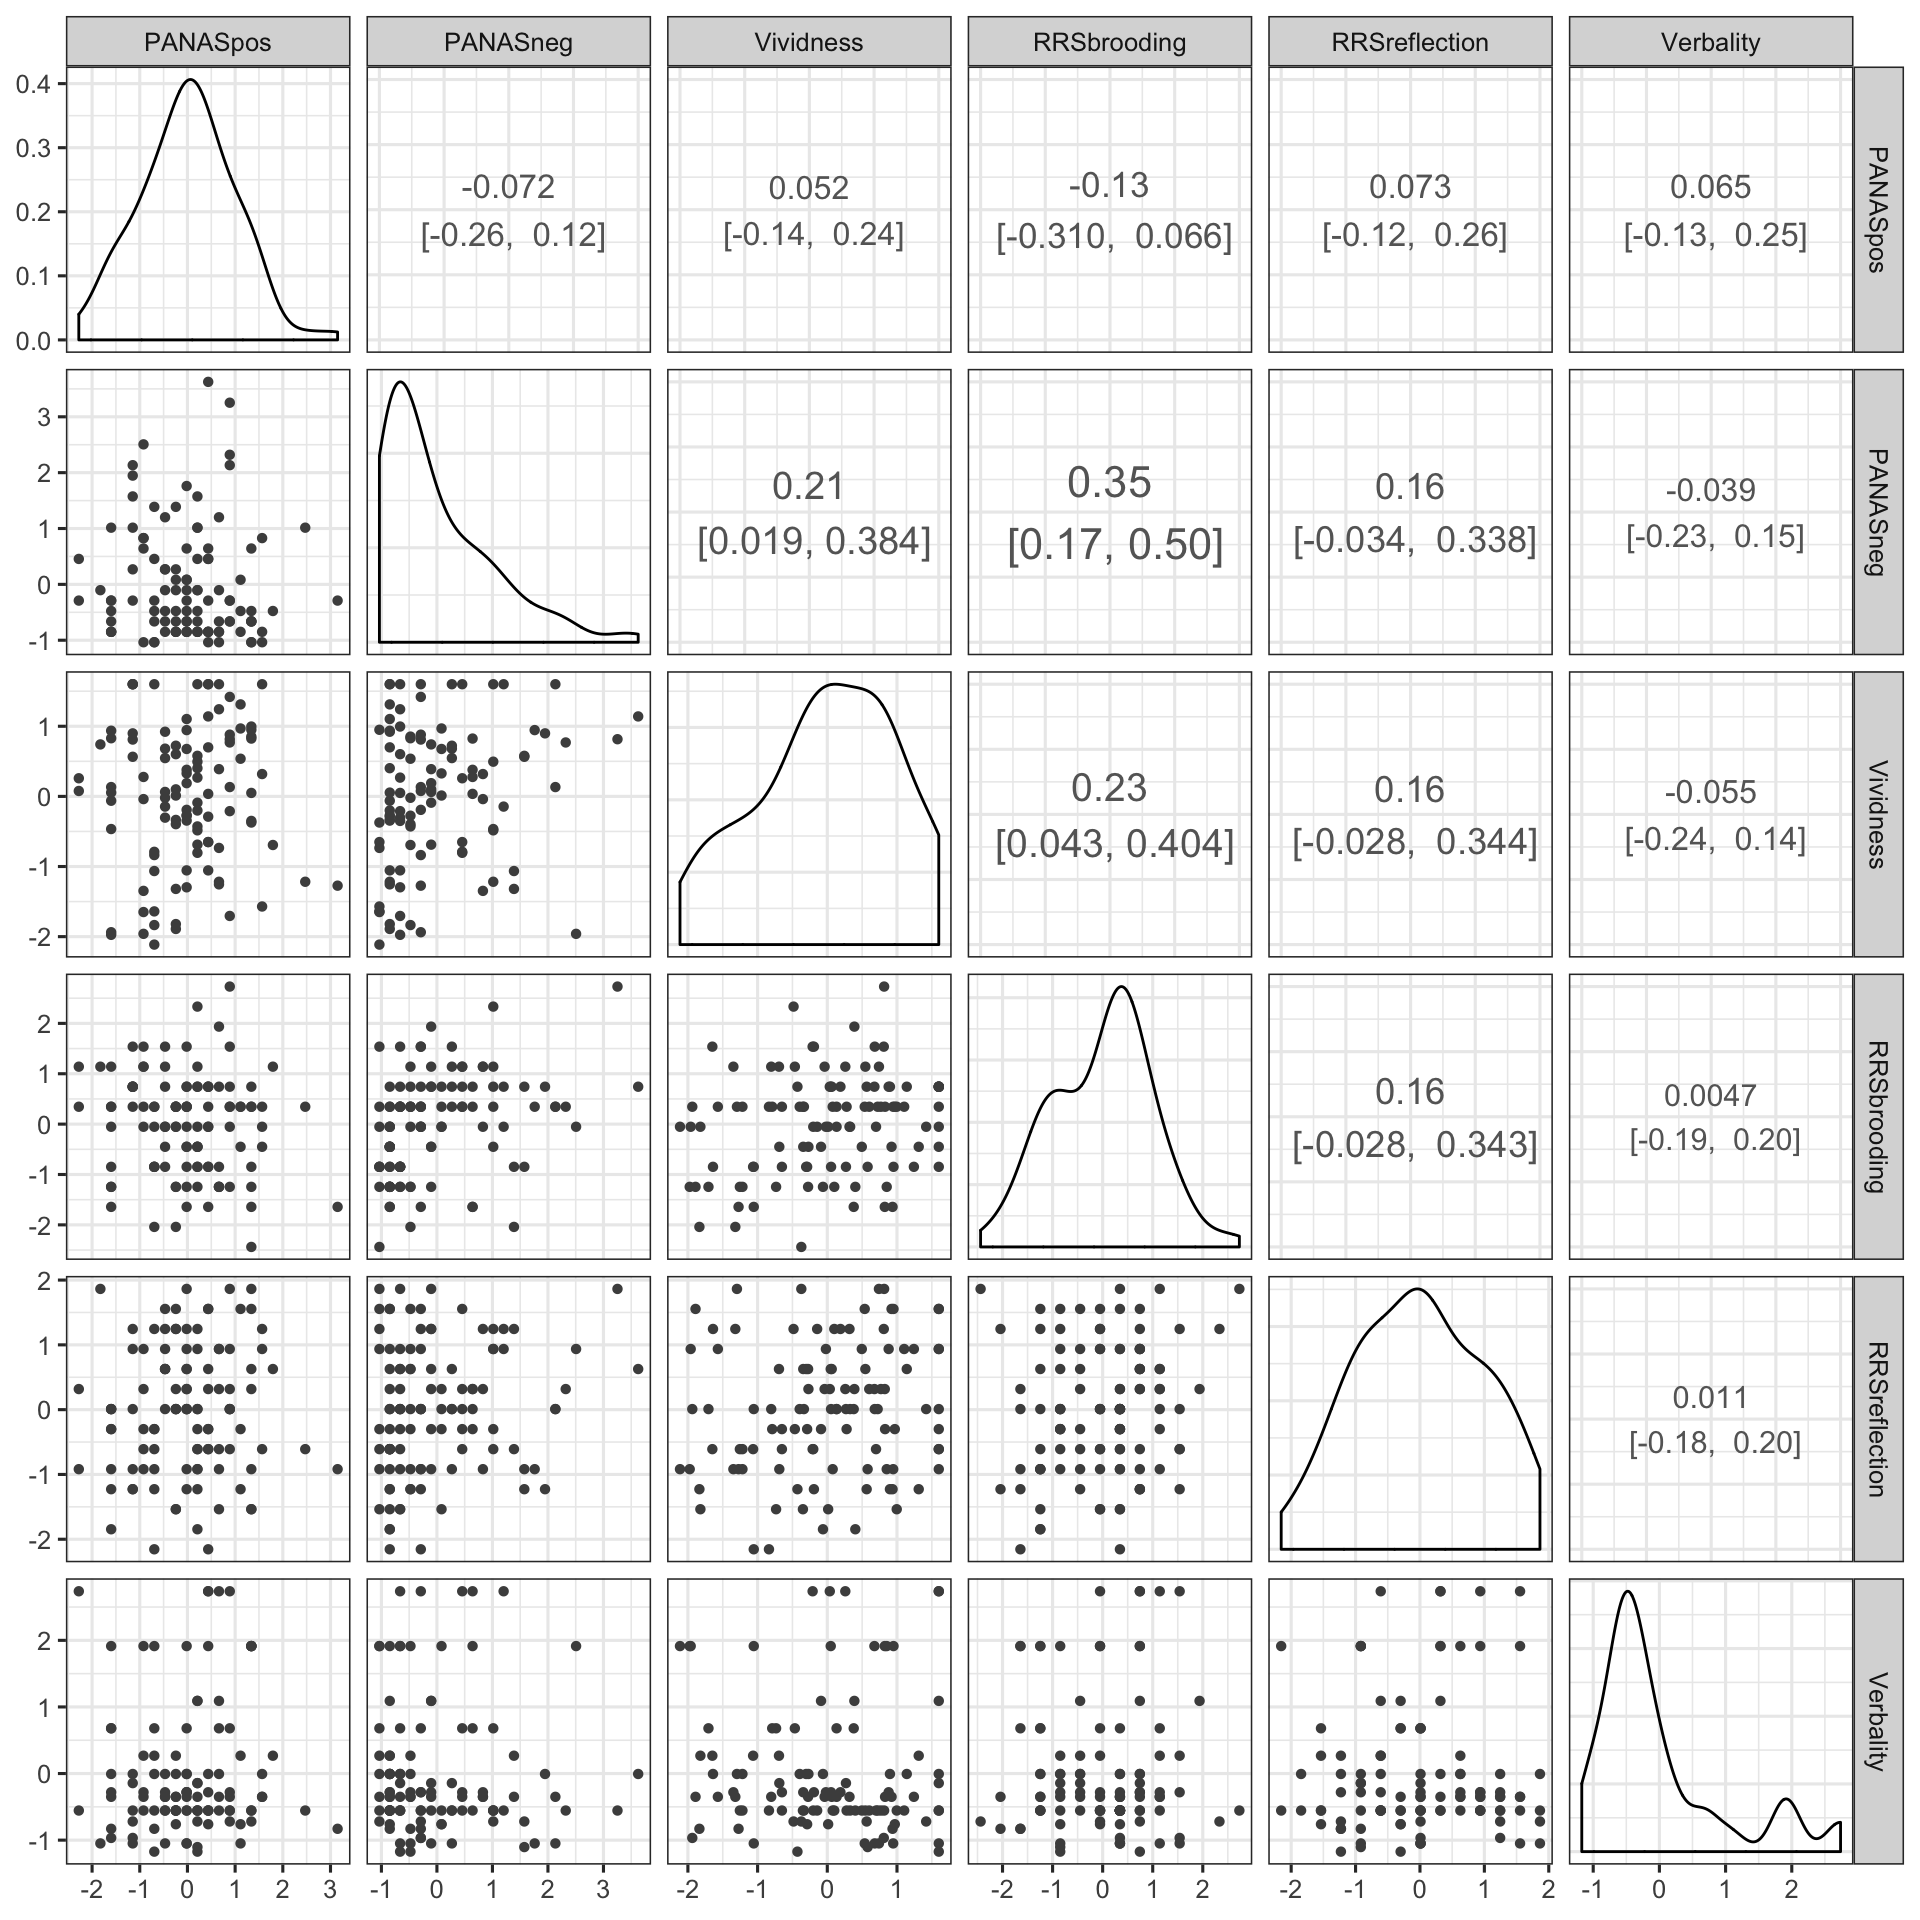
\includegraphics{06-chap6_files/figure-latex/correxp1-1.pdf}
\caption{\label{fig:correxp1}Diagonal: marginal distribution of each
variable. Panels above the diagonal: Pearson's correlations between main
continuous predictors, along with 95\% CIs. The absolute size of the
correlation coefficient is represented by the size of the text (lower
coefficients appear as smaller). Panels below the diagonal: scatterplot
of each variables pair.}
\end{figure}

\begin{table}

\caption{\label{tab:sumstat}Descriptive statistics (mean and standard deviation) of each recorded variable, for the final sample of participants that were included in the study.}
\centering
\begin{tabular}[t]{l|c|c|c|c|c|c}
\hline
Variables & Baseline & Post-induction & Post-motor & Baseline & Post-induction & Post-motor\\
\hline
RUM & 28.5 (26.49) & 54.66 (25.16) & 45.47 (27.25) & 20.96 (21.82) & 46.77 (25.74) & 43.54 (29.57)\\
\hline
Age & 20.3 (2.65) & - & - & 20.31 (2.53) & - & -\\
\hline
PANASneg & 15.65 (5.67) & - & - & 15.46 (5.08) & - & -\\
\hline
PANASpos & 30.91 (4.48) & - & - & 31.25 (4.4) & - & -\\
\hline
RRSbrooding & 12.2 (2.43) & - & - & 12.06 (2.62) & - & -\\
\hline
RRSreflection & 12.22 (3.22) & - & - & 11.71 (3.26) & - & -\\
\hline
Valence & 23.56 (22.4) & - & - & 37.53 (24.61) & - & -\\
\hline
Verbality & 1.67 (1.18) & - & - & 1.67 (1.26) & - & -\\
\hline
Vividness & 54.17 (28.94) & - & - & 59.78 (24.63) & - & -\\
\hline
\end{tabular}
\end{table}

\subsection{Rumination induction}\label{rumination-induction-2}

To examine the efficiency of the induction procedure (i.e., the effect
of \emph{Induction}) while controlling for the other variables (i.e.,
\emph{Vividness}, \emph{RRSbrooding}, \emph{RRSreflection},
\emph{PANASpos}, and \emph{PANASneg}), we then compared the parsimony of
models containing main constant effects and a varying intercept for
\emph{Participant}. Model comparison showed that the best model (in the
sense of the lowest AICc model) was the model including
\emph{Induction}, \emph{PANASpos}, \emph{PANASneg}, \emph{RRSbooding},
and an interaction term between \emph{Induction} and \emph{Vividness} as
predictors (see Table \ref{tab:compexp1}). Fit of the best model was
moderate as marginal \(R^{2}\) was of 0.3801215 while conditional
\(R^{2}\) was of 0.6838429.

\begin{table}

\caption{\label{tab:compexp1}Comparison of models, ordered by AICc relative to the model with the lowest AICc.}
\centering
\begin{tabular}[t]{l|l|c|c|c}
\hline
  & $K$ & $AICc$ & $\Delta_{AICc}$ & $Weight$\\
\hline
$Int+Ind+PANASpos+PANASneg+Ind:Viv+RRSbro$ & 8 & 1903 & 0 & 0\\
\hline
$Int+Ind+PANASpos+PANASneg+Ind:Viv+RRSref$ & 8 & 1903 & 0 & 0\\
\hline
$Int+Ind+PANASpos+PANASneg+Ind:Viv+RRSbro+RRSref$ & 9 & 1904 & 1 & 0\\
\hline
$Int+Ind+PANASneg+Ind:Viv$ & 6 & 1914 & 11 & 0\\
\hline
$Int+Ind+PANASneg$ & 5 & 1916 & 12 & 0\\
\hline
$Int+Ind+PANASpos+Ind:Viv$ & 6 & 1917 & 14 & 0\\
\hline
$Int+Ind+PANASpos$ & 5 & 1919 & 15 & 0\\
\hline
$Int+Ind+Ind:Viv$ & 5 & 1928 & 25 & 0\\
\hline
$Int+Ind$ & 4 & 1930 & 27 & 0\\
\hline
\end{tabular}
\end{table}

Constant effect estimates for the best model are reported in Table
\ref{tab:paramexp1}. Based on these values, it seems that
\emph{Induction} (i.e., the effects of the rumination induction)
increased \emph{RUM} scores by approximately 26 points in average
(\(d_{av} =\) 1.037, 95\% CI {[}0.748, 1.325{]}). The main negative
effect of \emph{PANASneg} and the main positive effects of
\emph{PANASpos} indicate, respectively, that negative baseline mood was
associated with higher levels of rumination while positive baseline mood
was associated with lower levels of self-reported rumination.

\textbackslash{}begin\{table\}

\textbackslash{}caption\{\label{tab:paramexp1}Coefficient estimates (Est),
standard errors (SE), and 95\% CIs (Lower, Upper).\} \centering

\begin{tabular}[t]{l|c|c|c|c}
\hline
 & Est & SE & Lower & Upper\\
\hline
(Intercept) & 37.796 & 1.859 & 34.153 & 41.438\\
\hline
Induction & 25.986 & 2.175 & 21.724 & 30.249\\
\hline
PANASpos & -6.805 & 1.877 & -10.485 & -3.126\\
\hline
PANASneg & 6.995 & 1.986 & 3.104 & 10.887\\
\hline
RRSbrooding & 2.688 & 1.997 & -1.225 & 6.601\\
\hline
Induction:Vividness & 4.273 & 2.178 & 0.003 & 8.542\\
\hline
\end{tabular}

\textbackslash{}end\{table\}

Higher scores on \emph{Vividness} were associated with higher increase
in self-reported rumination after induction, as revealed by the positive
coefficient of the interaction term. This suggests that participants who
recalled a more vivid negative memory tended to show a higher increase
in rumination after the induction procedure than participants with a
less vivid memory.

\section{Articulatory suppression effects on induced
rumination}\label{articulatory-suppression-effects-on-induced-rumination-1}

We then examined the effect of the two motor tasks (articulatory
suppression and finger-tapping) on \emph{RUM}, while controlling for
other variables (i.e., \emph{Vividness}, \emph{RRSbrooding},
\emph{RRSreflection}, \emph{Verbality}, \emph{PANASpos}, and
\emph{PANASneg}). Given the group differences on \emph{RUM} score at
baseline (i.e., after training), we also included this score as a
control variable in our models, as the \emph{RUMb} variable. Based on
our hypotheses, we expected that the model comparison would reveal a
three-way interaction between \emph{Session}, \emph{Condition} and
\emph{Verbality}. However, the best model identified by AICc model
comparison did not include this interaction as a constant effect.
Nonetheless, the best model was only slightly better than the model
including the three-way interaction (the second model in Table
\ref{tab:compexp2}), as the best model was only 1.1704261 more
\emph{credible} than the interaction model. As our goal is precise
estimation of effects rather than dichotomic decision about the presence
or absence of an effect, we chose to present the estimations of the
second model as well. Fit of this model was moderate as marginal
\(R^{2}\) was 0.2928069 while conditional \(R^{2}\) was 0.6626111.

\begin{table}

\caption{\label{tab:compexp2}Comparison of models, ordered by AICc relative to the model with the lowest AICc.}
\centering
\begin{tabular}[t]{l|l|c|c|c}
\hline
  & $K$ & $AICc$ & $\Delta_{AICc}$ & $Weight$\\
\hline
$Int+Session+Cond+RUMb+PANASneg+RRSbro+RRSref$ & 9 & 1914 & 0 & 0\\
\hline
$Int+Session+Cond+Session:Cond+RUMb+PANASneg+RRSbro+RRSref$ & 10 & 1914 & 0 & 0\\
\hline
$Int+Session+Cond+Session:Cond+Session:Cond:Verb+RUMb+PANASneg+RRSbro+RRSref$ & 11 & 1916 & 3 & 0\\
\hline
$Int+Session$ & 4 & 1947 & 33 & 0\\
\hline
$Int+Session+Cond$ & 5 & 1948 & 34 & 0\\
\hline
$Int+Session+Cond+Session:Cond$ & 6 & 1948 & 34 & 0\\
\hline
$Int+Session+Cond+Session:Cond:Verb$ & 7 & 1950 & 36 & 0\\
\hline
$Int$ & 3 & 1953 & 39 & 0\\
\hline
\end{tabular}
\end{table}

Parameter values of the best model for the second part of the experiment
are reported in Table \ref{tab:paramexp2}. Based on these values, it
seems that self-reported rumination decreased after both motor tasks
(the coefficient for \emph{Session} is negative), but this decrease was
substantially larger in the \emph{Mouthing} condition (\(d_{av} =\)
-0.351, 95\% CI {[}-0.735, 0.034{]}) than in the \emph{Tapping}
condition (\(d_{av} =\) -0.117, 95\% CI {[}-0.506, 0.273{]}), as can be
read from the coefficient of the interaction term between \emph{Session}
and \emph{Condition} (\emph{Est} = 5.965, \emph{SE} = 4.320, \emph{95\%
CI} {[}-2.502, 14.433{]}). However, the large uncertainty associated
with this result (as expressed by the width of the confidence interval)
warrants a careful interpretation of this result, that should be
considered as suggestive evidence, rather than conclusive evidence.

The large variation between participants can be appreciated by computing
the \emph{intra-class correlation} (ICC), expressed as
\(\sigma_{intercept}^{2}/(\sigma_{intercept}^{2}+\sigma_{residuals}^{2})\).
For the best model, the ICC is equal to 0.5229, indicating that 52.29\%
of the variance in the outcome that remains after accounting for the
effect of the predictors, is attributable to systematic inter-individual
differences.

\textbackslash{}begin\{table\}

\textbackslash{}caption\{\label{tab:paramexp2}Estimates (Est), standard
errors (SE), and 95\% CIs (Lower, Upper).\} \centering

\begin{tabular}[t]{l|c|c|c|c}
\hline
 & Est & SE & Lower & Upper\\
\hline
(Intercept) & 47.645 & 1.930 & 43.862 & 51.427\\
\hline
Session & -6.214 & 2.160 & -10.448 & -1.980\\
\hline
Condition & -0.948 & 3.921 & -8.633 & 6.736\\
\hline
RUMbaseline & 13.394 & 2.205 & 9.073 & 17.716\\
\hline
RRSbrooding & 2.449 & 2.088 & -1.643 & 6.541\\
\hline
RRSreflection & -2.039 & 1.981 & -5.921 & 1.843\\
\hline
PANASneg & 0.300 & 2.245 & -4.100 & 4.700\\
\hline
Session:Condition & 5.965 & 4.320 & -2.502 & 14.433\\
\hline
sd\_(Intercept).Participant & 16.462 & NA & NA & NA\\
\hline
sd\_Observation.Residual & 15.724 & NA & NA & NA\\
\hline
\end{tabular}

\textbackslash{}end\{table\}

Figure \ref{fig:plotexp1} shows the evolution of the mean \emph{RUM}
scores all through the experiment according to each session (Baseline,
Post-induction, Post-motor) and \emph{Condition} (Mouthing, Tapping).
This figure reveals important inter-individual variability, in all
conditions. After the rumination induction, \emph{RUM} score increased
in both groups, and decreased after the motor task, with a stronger
decrease in the \emph{Mouthing} condition.

\begin{figure}
\centering
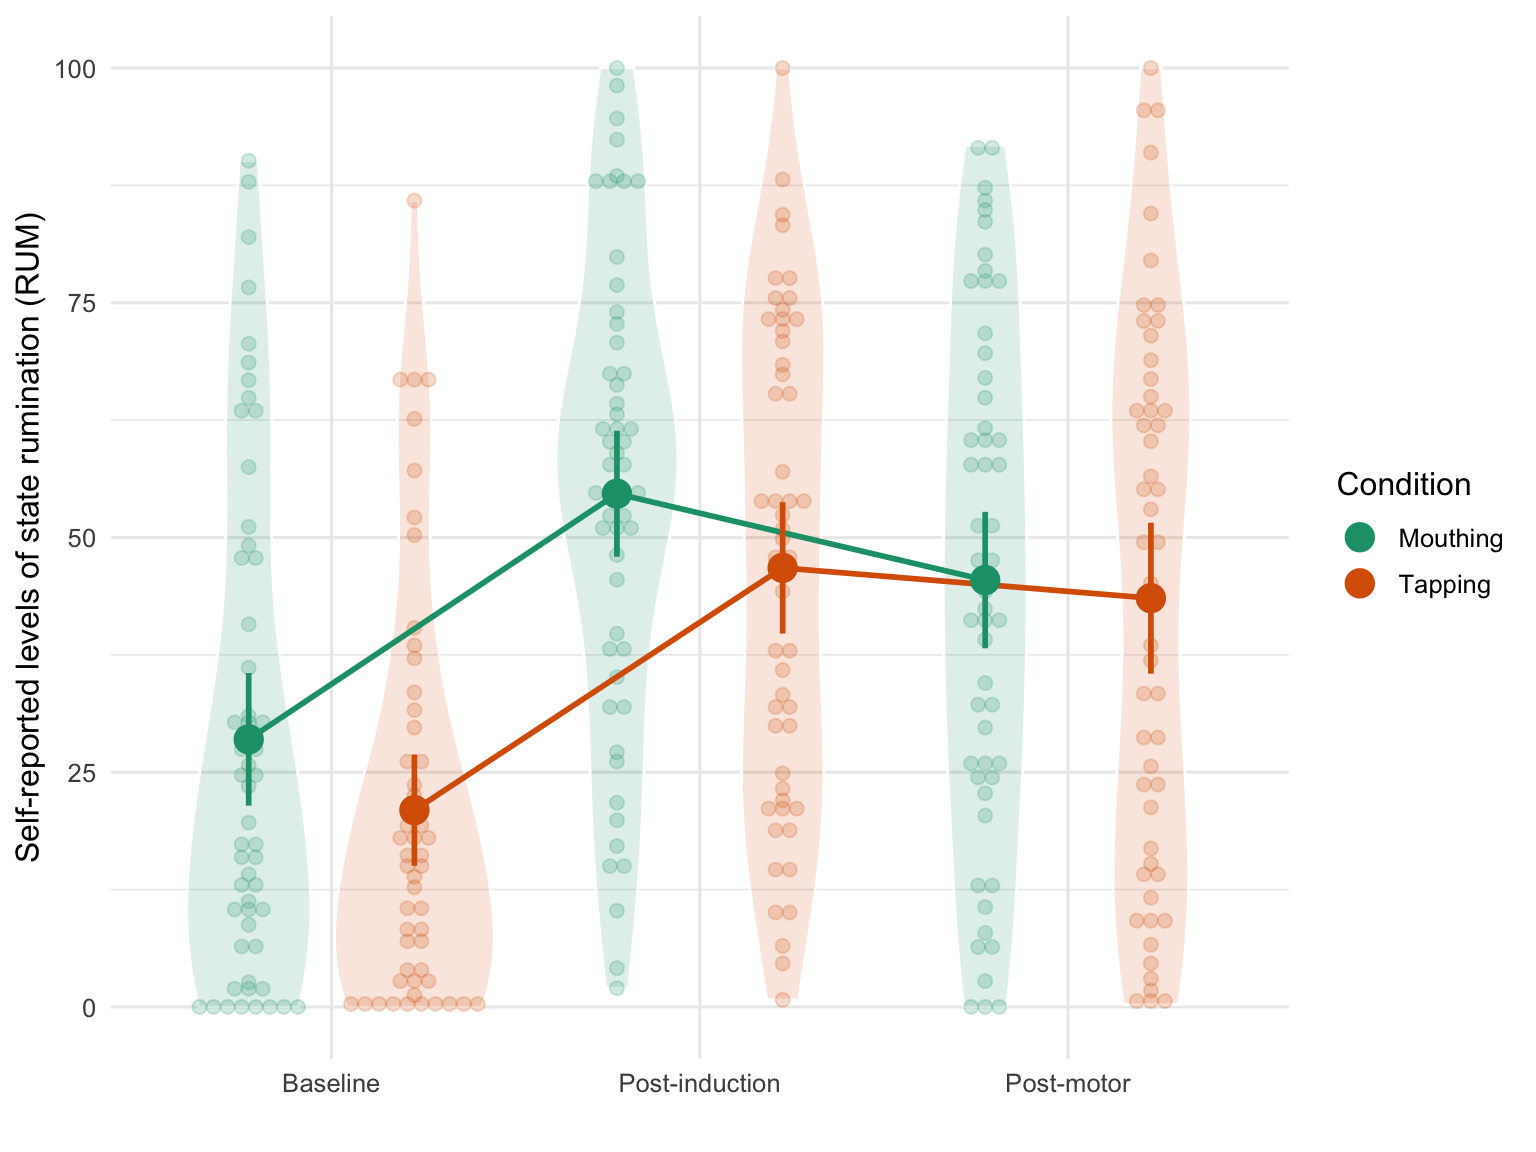
\includegraphics{06-chap6_files/figure-latex/plotexp1-1.pdf}
\caption{\label{fig:plotexp1}Mean RUM score by Session and Condition, along
with violin plots and individual data. Error bars represent 95\% CIs.
The horizontal bar inside the violin plots represents the median of the
conditional distribution.}
\end{figure}

Figure \ref{fig:plotverbal} shows the effects of \emph{Verbality} on the
relative change (i.e., after - before) in self-reported rumination after
both motor activities (i.e., \emph{Mouthing} and \emph{Tapping}). As
\emph{Verbality} was centered before analysis, its score cannot be
interpreted in absolute terms. However, a high score on this index
indicates more verbal than non-verbal (e.g., visual images, non-speech
sounds) thoughts, while a low score indicates more non-verbal than
verbal thoughts. Contrary to our predictions but consistent with the
model comparison, this figure depicts a similar relationship between
\emph{Verbality} and the change in \emph{RUM} score (between before and
after the motor task), according to the Condition.

\begin{figure}
\centering
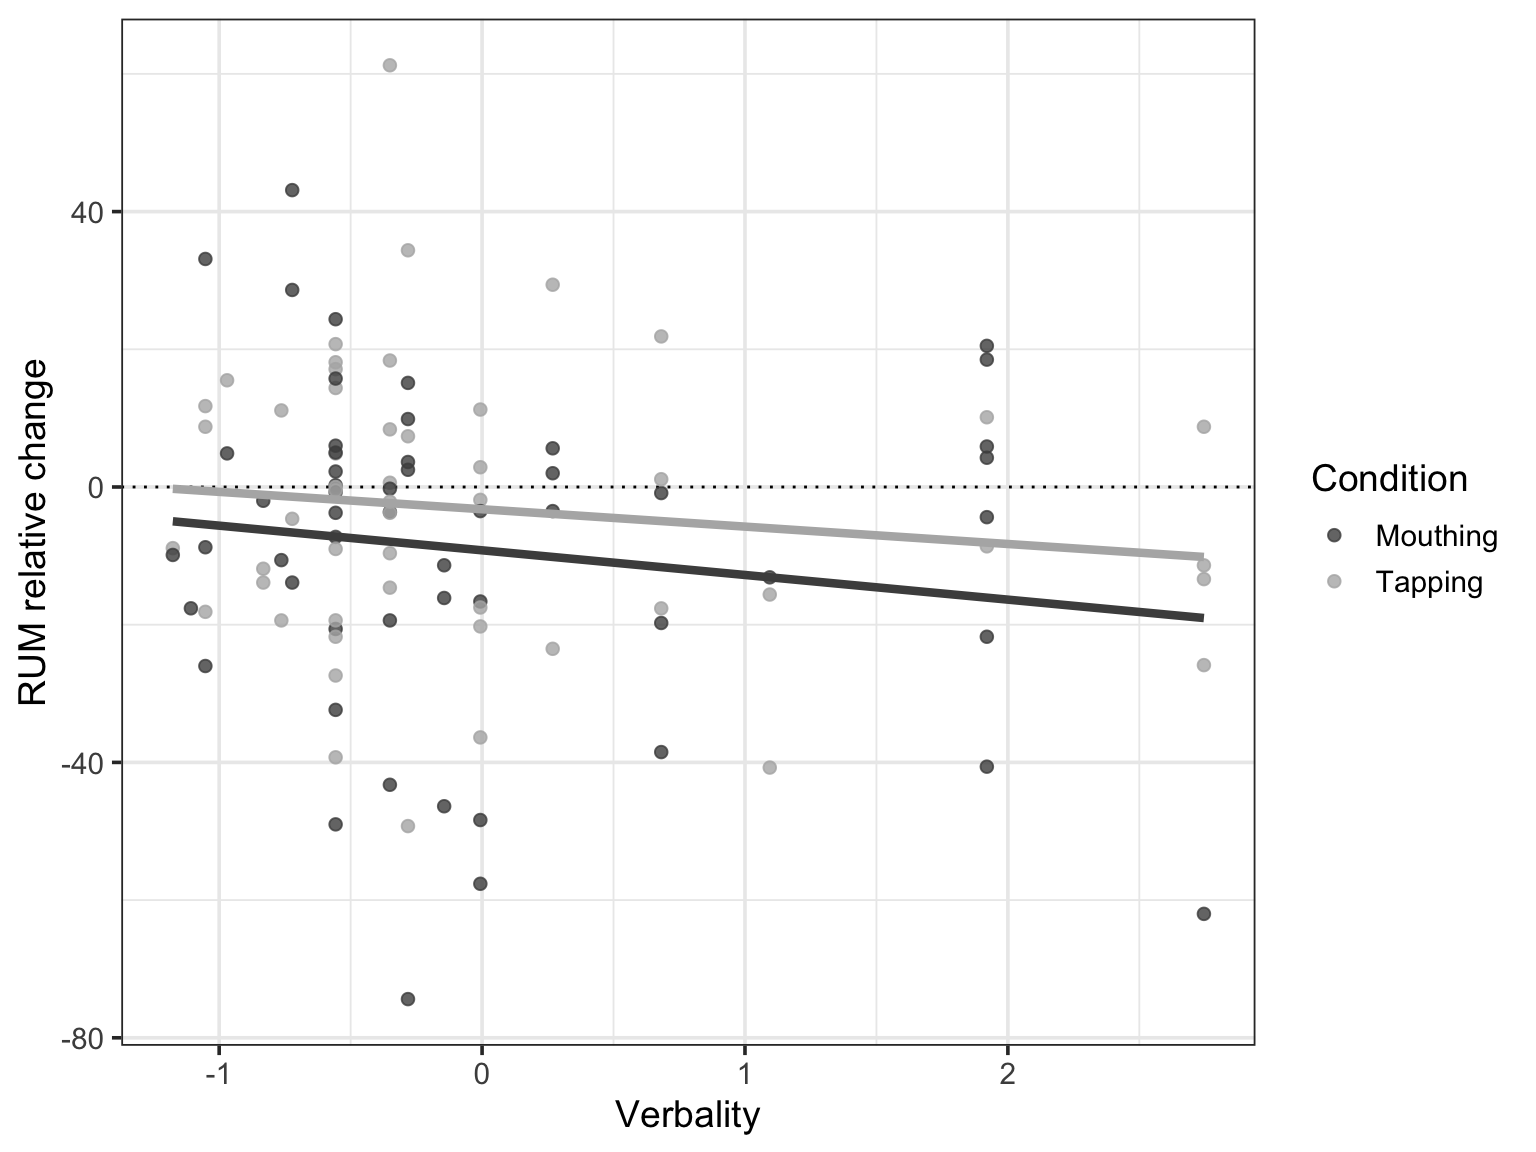
\includegraphics{06-chap6_files/figure-latex/plotverbal-1.pdf}
\caption{\label{fig:plotverbal}Mean RUM relative change after motor
activity, as a function of the degree of Verbality, in the mouthing (the
dark grey dots and regression line) and finger tapping (the light grey
dots and regression line) conditions.}
\end{figure}

\section{Discussion}\label{discussion}

The purpose of the current study was to investigate the effects of
articulatory suppression on induced verbal rumination. We predicted that
if verbal rumination, which can be construed as a type of inner speech,
does involve the mental simulation of overt speech production, its
generation should be disrupted by articulatory suppression, but not by
finger tapping. This prediction was not strictly corroborated by the
data, as we observed a decrease of self-reported rumination after both
types of motor activities (see Figure \ref{fig:plotexp1} and Table
\ref{tab:compexp2}), with a somewhat stronger decrease in the Mouthing
condition. In the following, we examine the validity of our methods and
discuss interpretations of our results. Finally, we formulate how
subsequent research should address this kind of question and suggest
alternative ways to test the above mentioned hypothesis. We begin by
discussing the results of the rumination induction procedure.

\subsection{Rumination induction}\label{rumination-induction-3}

It is noteworthy that 32.91\% of the total sample of participants who
were recruited did not respond to this induction, and were therefore not
included in the analyses. Moreover, as reported in Table
\ref{tab:paramexp1}, it seems that the \emph{Vividness} of the memory
chosen by the participant during the mood induction was moderating the
effect of the rumination induction. In other words, the more vivid
(i.e., the more ``intense'') the memory, the more successful the
rumination induction was. This highlights the fact that this aspect
should be carefully controlled each time a mood induction is used in
order to foster subsequent repetitive negative thinking.

Moreover, we observed a group difference of approximately 7.5 points in
the average \emph{RUM} score at baseline. This difference might be
explained by motor training, which took place before baseline
measurement of state rumination. During this training, participants had
to perform the motor task (either finger-tapping or mouthing) in front
of a screen on which a white dot was moving randomly on a black screen,
for 1 min. During the task, the experimenter stayed in the room (out of
the participant's sight) to check that participants were performing the
motor task adequately. Being an unusual and potentially embarrassing
motor activity, mouthing might have been an higher source of stress for
the participants, as compared to the more common activity of
finger-tapping. This group difference in baseline state rumination
subsisted after the induction, as the group difference after the
induction is of approximately 8 points (see full dataset and summary
statistics in the \protect\hyperlink{supp}{supplementary materials}).

\subsection{Articulatory suppression
effects}\label{articulatory-suppression-effects-1}

In the following section, we discuss in more depth the results of the
second part of the study, which aimed at comparing the effects of
articulatory suppression and finger-tapping on self-reported rumination.

First, it is important to examine whether our failure to detect the
predicted interaction could come from a lack of statistical power. We
planned 128 participants in order to reach a power of .80 for a targeted
effect size of \(\eta_{p}^{2}=.06\). As explained above, out of the 184
recruited participants, only 106 could be included in the study. With
106 participants, the a priori power was approximately of .70, which is
much higher than the median power in typical psychological studies.

Second, it is important to acknowledge that despite the absence of the
predicted difference between the two conditions in their influence on
the level of self-reported rumination (i.e., \emph{RUM}), both
activities did lead, on average, to a decrease in self-reported
rumination of approximately 6 points on the VAS (as indicated by the
slope for \emph{Session} in Table \ref{tab:paramexp2}). This decrease
might be interpreted in at least two ways. First, it might be explained
by the simple exposition to the VAS and by compliance effects. When
asked to rate their level of rumination again after five minutes of
motor activity, some participants might be prompted to indicate a lower
level of rumination than before the motor task. But compliance effects
could similarly lead participants to consider the motor task as
irritating, and therefore as prone to rumination increase. Some
participants could therefore also be biased towards indicating a higher
level of rumination after the motor task. Second, it might be considered
that this decrease reflects a genuine decrease in rumination. In the
following, we adopt the latter perspective and discuss explanations for
the weak difference between the two conditions.

\subsubsection{Effect of the rumination quality
(verbality)}\label{effect-of-the-rumination-quality-verbality}

Our prediction was that rumination in verbal form would be more
disrupted by mouthing than rumination in non-verbal form, while both
kinds of rumination would not be disrupted (or similarly disrupted) by
finger-tapping. In other words, we hypothesised a three-way interaction,
between the effect of time (i.e., \emph{Session}), \emph{Condition}, and
\emph{Verbality}. In the following, we discuss the absence of this
interaction. Then, we focus on the weak difference between the two
conditions (omitting \emph{Verbality}), and discuss some explanations
for this weak difference.

First, the absence of the three-way interaction might come from a
difficulty for the participants to have clear introspective access to
the ruminative thoughts they experienced during the experiment. For
instance, we know that introspective description of inner speech differs
considerably, between people trained to regularly report on their
episodes of inner speaking, and people without such training
\citep[e.g.,][]{Hurlburt2013}. Moreover, as the \emph{Verbality}
questionnaire was presented at the end of the experiment, one cannot
exclude that it was partly contaminated by recall, which, when done
verbally, has been shown to artificially increase the subjective
verbality index \citep{Hurlburt2011}.

\subsubsection{Difference between motor
conditions}\label{difference-between-motor-conditions}

Leaving the self-reported quality of rumination aside, we now turn to a
discussion of the weak difference between the two conditions. We think
this result can be explained in at least two non-exclusive ways. First,
we could argue that the decrease observed in both conditions was due to
an unexpected effect of finger-tapping on rumination. Second, we could
argue that the effect of the articulatory suppression was somehow weaker
than expected. In the following, we provide arguments and explanations
for each of these possibilities.

Steady finger-tapping is usually considered as a relevant control
condition for evaluating articulatory suppression, since it specifically
recruits the hand motor system and should not interfere with the oral
motor system, while being comparable in terms of general attentional
demands \citep[e.g.,][]{Gruber2001, Logie1987}. However, using more
complex rhythmic patterns of finger-tapping, \citet{Saito1994} observed
a fade-out of the phonological similarity effect in a verbal memory task
with spoken recall, when subjects were asked to tap with either their
right (dominant) or left hand, while the phonological similarity effect
was conserved in the control condition (no tapping). The author
concluded that a complex rhythmic tapping task can suppress the activity
of the articulatory control process, by \emph{suppressing} the running
of speech motor programs \citep[page 185]{Saito1994}. More specifically,
he suggested that complex, non-automatised, rhythmic finger tapping
could use speech motor programs, which are useful to control speech
prosody, and therefore can deal with rhythmic activity. We further
suggest that a novel complex rhythmic task might require silent
verbalisation and, therefore, might itself be an articulatory
suppression task. In line with these findings, another study showed that
for right-handed subjects, tapping with a finger of the right hand is
more effective at interfering with performance of a verbal memory task
than is tapping with a finger of the left hand \citep{Friedman1988}.
Although Friedman et al.'s findings are difficult to interpret, because
task priority was manipulated and this may have led to conflict
resolution, which might have been dealt with differentially according to
the hand involved, they do suggest that a finger tapping task is not
always the best control for articulatory suppression. This might explain
the decrease of self-reported rumination observed in our own study,
after the finger-tapping, and suggests that we might observe different
results by asking participants to tap with the finger of their
non-dominant hand. We think it is important to note for future studies
that our results, together with those of \citet{Saito1994} and
\citet{Friedman1988}, suggest that finger-tapping could in fact
interfere with inner speech. In other words, finger-tapping, with the
dominant hand, is probably not an appropriate control condition when
studying articulatory suppression.

As suggested previously, an alternative way to explain the absence of
differences between the two motor conditions is to suppose that the
effects of the articulatory suppression were weaker than we expected.
The rhythmic mouthing task might have become too automatised to disrupt
inner speech programming. This idea finds some support in the results of
\citet{Saito1997}, who observed an effect of articulatory suppression on
the phonological similarity effect in a memory task only when the
articulatory suppression was \emph{intermittent} (i.e., ``ah, ah,
ah\ldots{}'') but no effect when participants had to utter a continuous
``ah--''. This can be explained by considering that the intermittent
articulatory suppression would impose a greater load on speech motor
programming than the continuous articulatory suppression \citep[page
569]{Saito1997}. In a similar vein, \citet{Macken1995} found stronger
effects of articulatory suppression when participants were asked to
repeat a sequence of different letters than when they were asked to
repeat a single letter. One way to examine this hypothesis with our own
protocol would be to ask participants to make sequences of various mouth
movements, rather than repeating a single movement.

In a broader perspective, relating to the original research question, we
should mention two additional interpretations of our results. So far, we
considered different ways to explain either how the finger-tapping task
could interfere with rumination or how the articulatory suppression task
might have failed to disrupt rumination. However, if we assume that our
scales (especially the \emph{RUM} outcome response and the
\emph{Verbality} scale) are reliable and that the articulatory
suppression was efficient in its intended purpose, we are forced to
admit that either i) rumination is not a type of inner speech that can
be disrupted by peripheral muscle perturbation (i.e., it could be
described as a more abstract form of inner speech) or that ii) inner
speech, more broadly, does not depend on peripheral speech muscle
activity. Although we think that these questions cannot be answered from
our present results, we acknowledge that these two possibilities are
compatible with our results.

In summary, the current research is one of the first behavioral studies
exploring the association between verbal rumination and the speech motor
system. While the observed data did not strictly corroborate our
original hypotheses, we explored several explanations for the weak
difference between articulatory suppression and the control task, and
related our findings to previous works on the role of inner speech in
verbal working memory. These results have important implications for
future studies on articulatory suppression during inner speech or
working memory tasks. More precisely, they highlight the need for
further investigation of the most appropriate control task when studying
the effects of articulatory suppression.

\hypertarget{supp}{\section*{Supplementary materials}\label{supp}}
\addcontentsline{toc}{section}{Supplementary materials}

Pre-registered protocol, preprint, data, as well as reproducible code
and figures are available at: \href{http://osf.io/3bh67}{osf.io/3bh67}.

A lot of useful packages have been used for the writing of this paper,
among which the \texttt{papaja} and \texttt{knitr} packages for writing
and formatting \citep{R-papaja, R-knitr}, the \texttt{ggplot2},
\texttt{ggforce}, \texttt{GGally}, \texttt{DiagrammeR}, and
\texttt{plotly} packages for plotting
\citep{R-ggplot2, R-ggforce, R-GGally, R-DiagrammeR, R-plotly}, the
\texttt{AICcmodavg}, and \texttt{Rmisc} packages for data analysis
\citep{R-AICcmodavg, R-Rmisc}, as well as the \texttt{tidyverse} and
\texttt{broom} packages for code writing and formatting
\citep{R-broom, R-tidyverse}.

\section*{Acknowledgements}\label{acknowledgements}
\addcontentsline{toc}{section}{Acknowledgements}

This project was funded by the ANR project INNERSPEECH (grant number
ANR-13-BSH2-0003-01). The first author of the manuscript is funded by a
fellowship from Université Grenoble Alpes. We thank David Meary for his
technical support in programming the eye-tracking experiment. We thank
Rafael Laboissiere and Brice Beffara for their advice concerning data
analysis.

\section*{Appendix A. Eye-tracking control
experiment}\label{appendix-a.-eye-tracking-control-experiment}
\addcontentsline{toc}{section}{Appendix A. Eye-tracking control
experiment}

The purpose of this control experiment was to demonstrate that the two
motor tasks used in the main experiment, namely, finger tapping and
articulatory suppression (mouth movements) were equivalent in terms of
task difficulty or general dual-task demand \citep{Emerson2003}.
Participants performed a computer-based visual search task (i.e.,
finding a T among an array of Ls), adapted from the \citet{Treisman1980}
paradigm (see below for details).

\subsection*{Sample}\label{sample-1}
\addcontentsline{toc}{subsection}{Sample}

Twenty-four participants (Mean age = 19.46, SD = 1.18, Min-Max = 18-21,
21 females, 21 right-handed), drawn from the same population (i.e.,
undergraduate psychology students) as the main experiment took part in
this eye-tracking pretest.

\subsection*{Sample size}\label{sample-size}
\addcontentsline{toc}{subsection}{Sample size}

As we aimed to compare four conditions (i.e., visual search (VS) task
alone, VS + finger tapping, VS + foot tapping and VS + mouth movements),
we recruited 24 participants in order to have at least one participant
per order in our random counter-balanced repeated measures design
(\(n = k!\) where \(n\) is the number of possible orders of conditions
for \(k\) conditions, then \(n =4 != 24\)).

\subsection*{Material}\label{material-1}
\addcontentsline{toc}{subsection}{Material}

Experiment took place individually in a dark room. Participants had to
seat in front of a 22 inches, Iyama Vision Master Pro 513-MA203DT CRT
Monitor (resolution: 1024x768 pixels, refresh rate: 85 Hz) with a NVIDIA
GeForce 9800 GTX+ graphic processor. A camera-based eye-tracker
(EyeLink\textregistered~1000 from SR Research) with a sampling rate of
250 Hz and a minimum accuracy of 0.5° was used, in the pupil-corneal
reflection tracking mode. Participants were positioned on a seat so as
to keep distance from the camera to the forehead target between 50 and
60 cm. A five-point calibration was completed before presenting stimuli,
at the beginning of each condition.

\subsection*{Procedure}\label{procedure-1}
\addcontentsline{toc}{subsection}{Procedure}

The target (i.e., the letter ``T'') was present at each trial, either on
the right or on the left of the central vertical axis of the grid. The
grid was an array of 6*6 items. Each stimulus was displayed until the
participant response (maximum duration in case of no response: 5
seconds). Each grid of letters was preceded by a central fixation
circle, that was displayed for 500ms after the participant moved his/her
gaze towards it. In order to give their response (``left'' or
``right''), participants had to gaze towards a large filled gray circle,
situated either on the left or on the right side of the grid. Each
participant went through each condition, in a random order. A first
general training session was proposed, at the beginning of the
experiment, using ten items that were not used subsequently in the four
conditions. Each condition was composed of 90 trials (45 left and 45
right), knowing that the first ten trials of each condition were
considered as training trials and thus not included in analysis. All
participants were filmed in order to ensure that they effectively
performed the motor activity. Our measure of interest was the delay
between the apparition of the grid and the participant's response (the
time at which his/her gaze reached the response circle), below referred
to as ``response time'' (RT).

\subsection*{Data preprocessing}\label{data-preprocessing}
\addcontentsline{toc}{subsection}{Data preprocessing}

Raw data from EyeLink\textregistered~includes gaze on screen spatial
coordinates, pupil diameter and forehead target spatial coordinates,
with its distance from the camera. For this experiment, since only RTs
(in ms) of correct trials are interesting, invalid trials (when no
response has been given) and wrong responses were removed from the
analysis.

\subsection*{Data analysis}\label{data-analysis-1}
\addcontentsline{toc}{subsection}{Data analysis}

Data were analysed using \emph{Condition} (4 modalities) as a
within-subject predictor and the natural logarithm of the RT as a
dependent variable in a MLM, including a varying intercept for both
\emph{participant} and \emph{item}. Comparisons of interest were
computed using Helmert contrasts. Estimates and confidence intervals are
reported for each comparison in the log scale.

\subsection*{Results}\label{results-1}
\addcontentsline{toc}{subsection}{Results}

Results of the MLM are reported in Table \ref{tab:paramET} and Figure
\ref{fig:eyetrack}. Contrast analysis revealed a slight difference
between the \emph{Control} condition and the mean of the three other
conditions (Est = -0.0099591, 95\% CI = {[}-0.015235, -0.0046832{]}) as
well as a slight difference between the \emph{Foot} condition and the
mean of the \emph{Finger} and the \emph{Mouth} conditions (Est =
0.0050298, 95\% CI = {[}-0.0024395, 0.0124992{]}) while no apparent
differences between the \emph{Mouth} and the \emph{Finger} conditions
(Est = -0.0063662, 95\% CI = {[}-0.0192938, 0.0065614{]}).

\begin{table}

\caption{\label{tab:paramET}Coefficient estimates (Est), standard errors (SE), and 95\% CIs (Lower, Upper) of each contrast.}
\centering
\begin{tabular}[t]{l|c|c|c|c}
\hline
 & $Est$ & $SE$ & $Lower$ & $Upper$\\
\hline
$Control\ vs\ all$ & -0.00996 & 0.00269 & -0.01524 & -0.00468\\
\hline
$Foot\ vs\ Finger + Mouth$ & 0.00503 & 0.00381 & -0.00244 & 0.01250\\
\hline
$Finger\ vs\ Mouth$ & -0.00637 & 0.00660 & -0.01929 & 0.00656\\
\hline
\end{tabular}
\end{table}

\begin{figure}
\centering
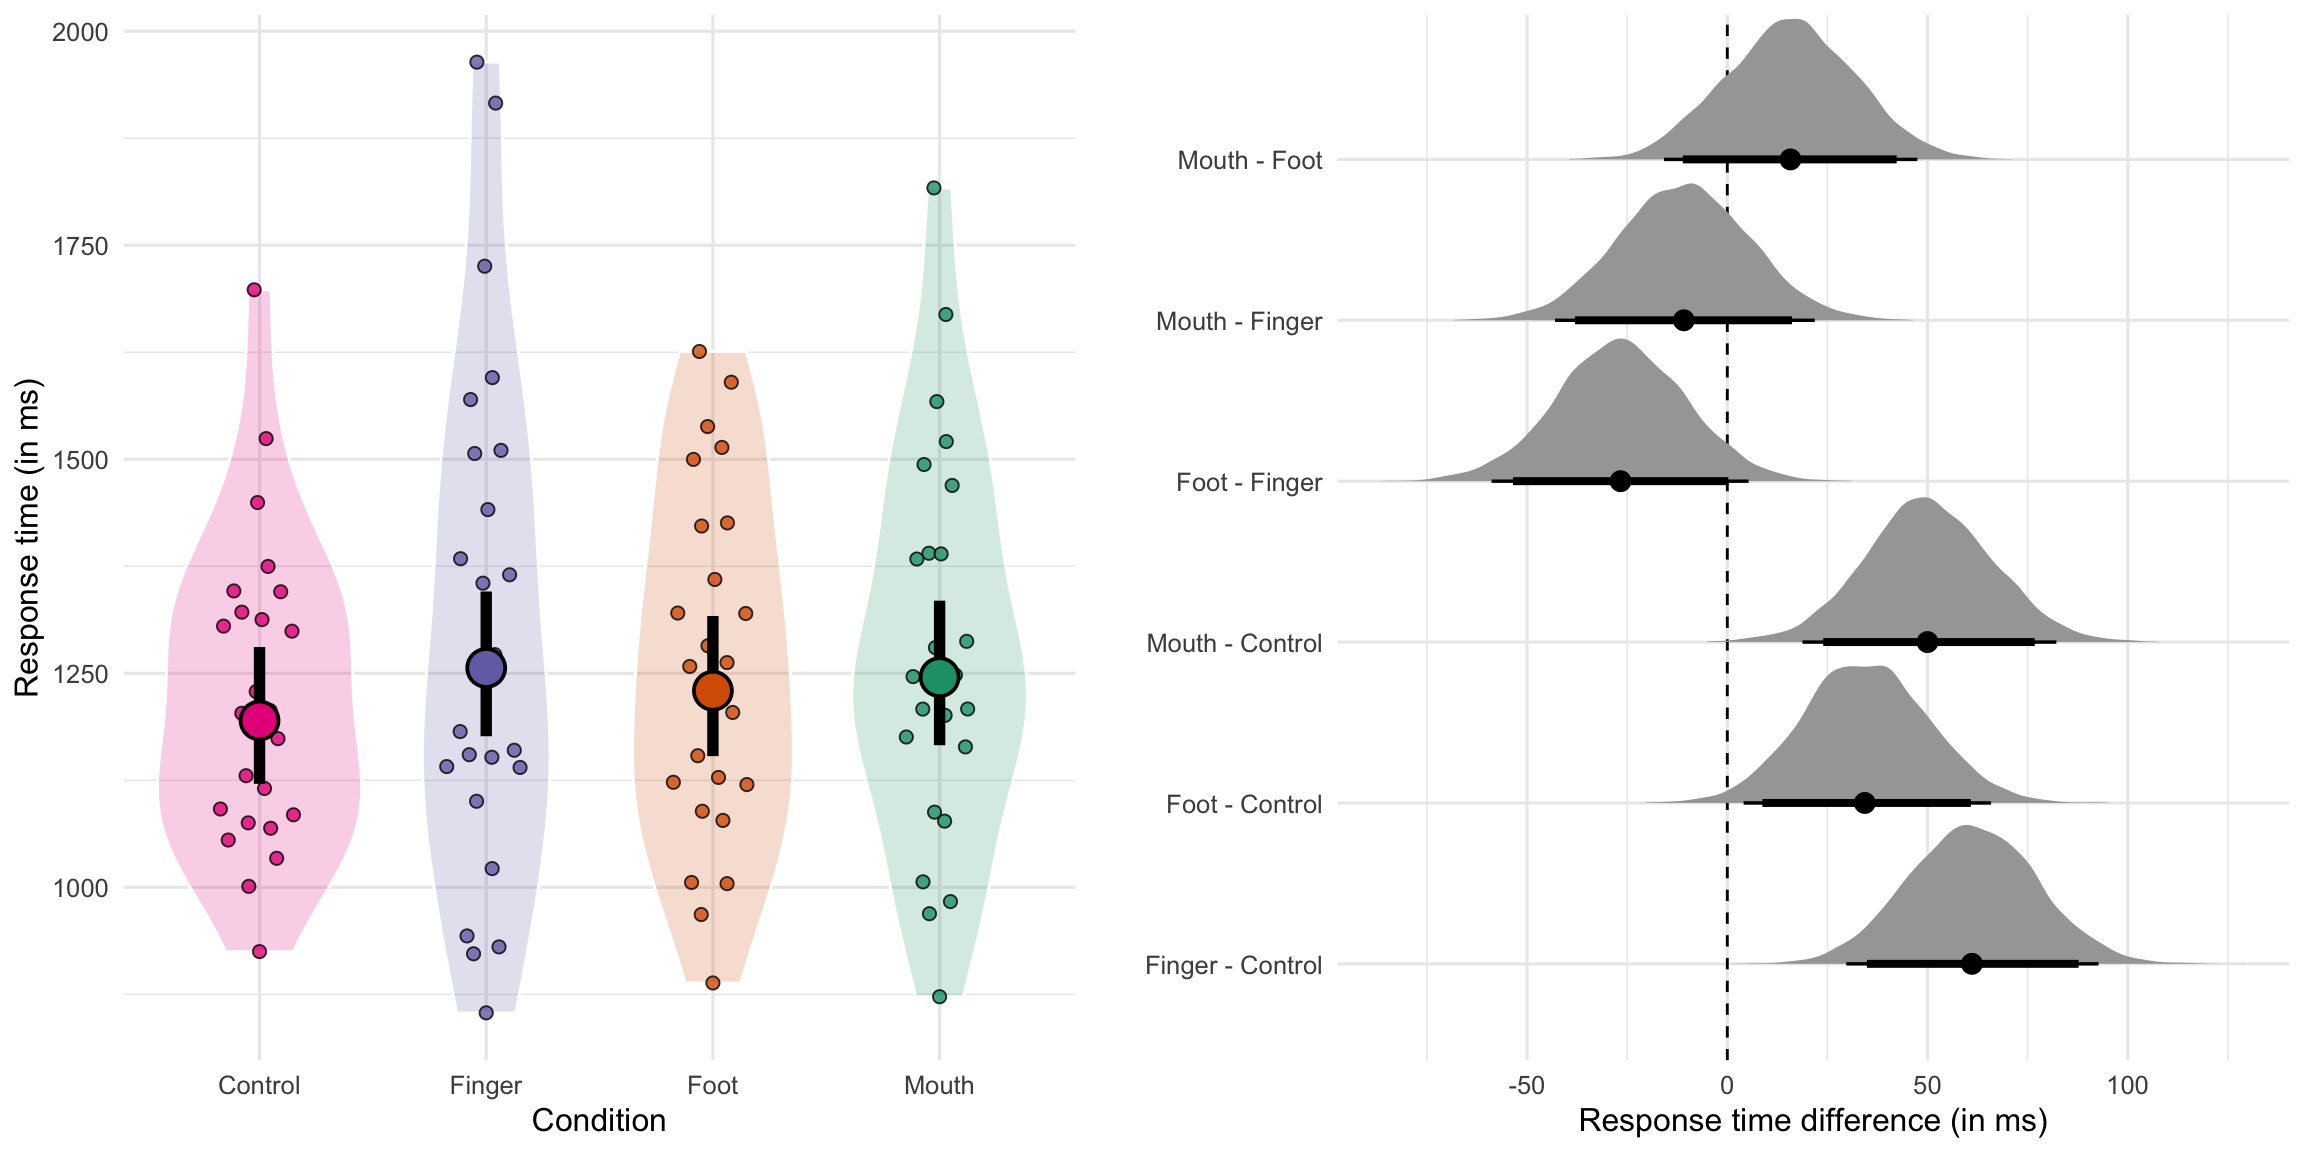
\includegraphics{06-chap6_files/figure-latex/eyetrack-1.pdf}
\caption{\label{fig:eyetrack}Mean RTs by Condition along with 95\% CIs and
violin plots (the horizontal line represents the median of the
conditional distribution). Grey dots represent mean RTs by participant.}
\end{figure}

\subsection*{Discussion}\label{discussion-1}
\addcontentsline{toc}{subsection}{Discussion}

This control experiment shows that there is no apparent difference (or a
negligible one) in terms of attentional demand between the two motor
tasks used in the main experiment (i.e., finger-tapping and mouthing),
although performing a dual motor task (of any type) does seem costly,
because of the observed difference between the control condition and the
mean of the three others conditions. These results are in line with the
results obtained by \citet{Cefidekhanie2014} in their control
experiment.

\chapter{TMS study}\label{tms-study}

\ldots{}

\part{General discussion and
conclusions}\label{part-general-discussion-and-conclusions}

\chapter{General discussion}\label{general-discussion}

\ldots{}

\chapter{Conclusions}\label{conclusions}

\ldots{}

\noindent
\setlength{\parindent}{-0.20in} \setlength{\leftskip}{0.20in}
\setlength{\parskip}{8pt}

\bibliography{bib/book.bib,bib/packages.bib}


\end{document}
